\documentclass[10pt,a4paper]{article}
%\documentclass[aps,prl]{revtex4-1}
\usepackage[margin=2.5cm,footskip=1.cm,includefoot]{geometry}% spremenimo sirine robov
\usepackage{floatrow}
\usepackage{hyperref}
\usepackage{amsmath}
\usepackage{fullpage}
\usepackage{amsfonts}
\usepackage{amssymb}
\usepackage{lmodern}
\usepackage{url}
\usepackage[labelformat=simple,font=small]{subcaption}
\usepackage[font=small]{caption}
%\usepackage{subcaption}
\usepackage[multiple]{footmisc}
\usepackage[]{units}
\usepackage{bm}
\usepackage{fancyhdr}
%\usepackage[demo]{graphicx}
\usepackage{graphicx}
\usepackage{mhchem}
\newcommand{\iu}{{i\mkern1mu}}

\addtolength\hoffset{0.5cm}%horizontalni premik
%vse pametne funkcije ki jih lahko rabimo (lahko tudi kopiras direktno zraven)
\setlength{\parindent}{0pt}%ni pomika za paragrafe
\setlength{\parskip}{0.75ex}%med paragrafi je malo lufta

\usepackage[pdftex]{graphicx}%za slike: predvidimo da bomo klicali pdflatex.

\usepackage{amsmath}
\usepackage{amsfonts}
\usepackage{mathrsfs}
\usepackage[usenames]{color}
\usepackage[slovene]{babel}
\usepackage[utf8]{inputenc}%to omogoca uporabo sumnikov. Brez tega rabis \v{c}, \v{s}, \v{z} in vse ostalo.

%nekaj koristnih funkcij.
\newcommand{\HRule}{\rule{\linewidth}{0.5mm}}   %debela črta čez celo stran

\newcommand{\ve}[1]{\ensuremath{\mathbf{#1}}} % for vectors
\newcommand{\gv}[1]{\ensuremath{\mbox{\boldmath$ #1 $}}} 
% for vectors of Greek letters
\newcommand{\uv}[1]{\ensuremath{\mathbf{\hat{#1}}}} % for unit vector
\newcommand{\abs}[1]{\left| #1 \right|} % for absolute value

\renewcommand{\Re}{\mathop{\rm Re}}
\renewcommand{\Im}{\mathop{\rm Im}}
\newcommand{\Tr}{\mathop{\rm Tr}}
\newcommand{\dd}{\,\mathrm{d}}
\newcommand{\ddd}{\mathrm{d}}
\newcommand{\ii}{\mathrm{i}}
\newcommand{\lag}{\mathcal{L}\!}
\newcommand{\ham}{\mathcal{H}\!}
\newcommand{\four}[1]{\mathcal{F}\!\left(#1\right)}
\newcommand{\bigO}[1]{\mathcal{O}\!\left(#1\right)}
\newcommand{\sh}{\mathop{\rm sinh}}
\newcommand{\ch}{\mathop{\rm cosh}}
\renewcommand{\th}{\mathop{\rm tanh}}
\newcommand{\erf}{\mathop{\rm erf}}
\newcommand{\erfc}{\mathop{\rm erfc}}
\newcommand{\sinc}{\mathop{\rm sinc}}
\newcommand{\rect}{\mathop{\rm rect}}
\newcommand{\ee}[1]{\cdot 10^{#1}}
\newcommand{\inv}[1]{\left(#1\right)^{-1}}
\newcommand{\invf}[1]{\frac{1}{#1}}
\newcommand{\sqr}[1]{\left(#1\right)^2}
\newcommand{\half}{\frac{1}{2}}
\newcommand{\thalf}{\tfrac{1}{2}}
\newcommand{\pd}{\partial}
\newcommand{\Dd}[3][{}]{\frac{\ddd^{#1} #2}{\ddd #3^{#1}}}
\newcommand{\DD}[3][{}]{\frac{D^{#1} #2}{D #3^{#1}}}
\newcommand{\Pd}[3][{}]{\frac{\pd^{#1} #2}{\pd #3^{#1}}}
\newcommand{\bra}[1]{\langle #1 \vert}
\newcommand{\ket}[1]{\vert#1\rangle}
\newcommand{\avg}[1]{\left\langle#1\right\rangle}
\newcommand{\norm}[1]{\left\Vert #1 \right\Vert}
\newcommand{\braket}[2]{\left\langle #1 \vert#2 \right\rangle}
\newcommand{\obraket}[3]{\left\langle #1 \vert #2 \vert #3 \right \rangle}
\newcommand{\en}[1]{\mathop{\rm #1}}
\newcommand{\hex}[1]{\texttt{0x#1}}

\renewcommand{\iint}{\mathop{\int\mkern-13mu\int}}
\renewcommand{\iiint}{\mathop{\int\mkern-13mu\int\mkern-13mu\int}}
\newcommand{\oiint}{\mathop{{\int\mkern-15mu\int}\mkern-21mu\raisebox{0.3ex}{$\bigcirc$}}}

\newcommand{\wunderbrace}[2]{\vphantom{#1}\smash{\underbrace{#1}_{#2}}}


\renewcommand{\vec}[1]{\overset{\smash{\hbox{\raise -0.42ex\hbox{$\scriptscriptstyle\rightharpoonup$}}}}{#1}}
\newcommand{\bec}[1]{\mathbf{#1}}

%\pagestyle{plain}
\pagestyle{headings}

\usepackage{titlesec}
\usepackage{cleveref}
\renewcommand{\thesubfigure}{(\alph{subfigure})}
\captionsetup[sub]{labelformat=simple}

\titleformat*{\section}{\Large\bfseries}
\titleformat*{\subsection}{\large\bfseries}
\titleformat*{\subsubsection}{\large\bfseries}
\titleformat*{\paragraph}{\large\bfseries}
\titleformat*{\subparagraph}{\large\bfseries}

\usepackage{color}

\pagenumbering{arabic}

\begin{document}
%%% NASLOVNA STRAN


\begin{center}

% 
\includegraphics[width=0.35\textwidth]{logo_fmf_uni-lj_en.pdf}\\[8ex] 

\vspace{3mm}


%{\large }\\
\vspace{2 cm}

{ \Large }Magistrsko delo\\             
\vspace{3cm}


{\large Avtor: Jan Šuntajs\\
\large Mentor: dr. Janez Bonča \\
\large Mentor: doc. Lev Vidmar 
\vspace{2cm}



Ljubljana, 2017}
\vfill
\begin{abstract}

\end{abstract}

\end{center}

\cleardoublepage

\thispagestyle{empty}


%\tableofcontents
\clearpage
\pagestyle{fancy}
\fancyhf{}
\cfoot{\thepage}
\setcounter{page}{1}

\section{Uvod}
%VIRI: NANDKISHORE, HUSE, UVOD
%ABANIN, UVOD
%MONDAINI, RIGOL (za stil pisanja pri nanašanju na Andersona)
Nastop \emph{večdelčne lokalizacije} (ang. \emph{many-body localization}, v nadaljevanju MBL) v izoliranih neurejenih kvantnomehanskih sistemih s prisotnostjo meddelčnih interakcij vodi do osupljivih lastnosti tovrstnih sistemov. Med njimi je poglavitna in najočitnejša odsotnost termalizacije, sicer značilne za generične večdelčne sisteme z ergodično dinamiko. V termodinamski limiti unitaren dolgočasovni razvoj poljubnih začetnih stanj ergodičnih sistemov vodi do ravnovesja, v katerem pričakovane vrednosti kvantnomehanskih opazljivk podajajo ustrezna kvantnomehanska ansambelska povprečja. Zaradi odsotnosti sklopitve z zunanjim rezervoarjem je tovrstna relaksacija neravnovesnih začetnih stanj proti ravnovesnim termalnim vrednostim v izoliranem sistemu možna le, če sistem sam sebi predstavlja `efektivno toplotno kopel'. To pomeni, da se mora podsistem z makroskopsko zanemarljivim deležem prostostnih stopenj  celotnega sistema s preostankom sistema sklapljati podobno, kot se v običajni formulaciji statističnomehanskih ansamblov sistemi sklapljajo z zunanjim rezervoarjem~\cite{abanin2018ergodicity}~\cite{nandkishore2015many}. \\
\begin{minipage}[t]{0.42\textwidth}
\noindent \\
Skupaj z integrabilnimi sistemi predstavljajo MBL sistemi pomemben protiprimer
zgoraj opisani dinamiki ergodičnih sistemov, kar je shematsko predstavljeno na Sliki~\ref{fig:abanin_thermalization}. Prikazan je časovni razvoj netipičnega začetnega profila kvantnomehanske opazljivke, točneje gostote delcev, v ergodičnem in MBL primeru. Medtem ko pri prvem pričakovane vrednosti lokalnih opazljivk po dolgem času določajo vrednosti ansambelskih povprečij, ki so odvisne le od nekaj dobro definiranih makroskopskih količin, denimo energije in števila delcev, je obnašanje MBL sistemov popolnoma drugačno. `Spomin' na netipičnost začetne konfiguracije se namreč v pričakovanih vrednostih lokalnih opazljivk ohrani tudi po 
\end{minipage}\hfill
\begin{minipage}[t]{0.55\textwidth}
\begin{figure}[H]
\centering{
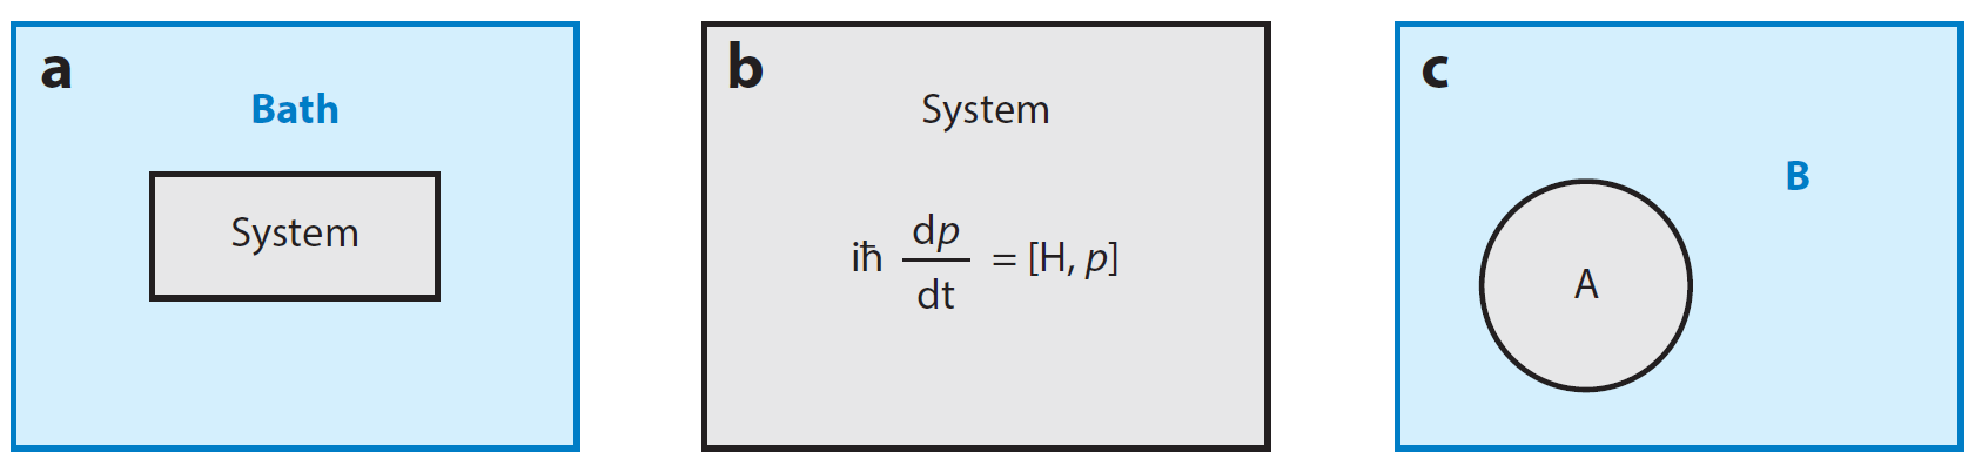
\includegraphics[width=1\textwidth]{nandkishore_huse_reservoir.pdf}}
\caption{
\textbf{a)} Pri običajnem kvantnostatističnem opisu sistema privzamemo njegovo sklopitev z zunanjim rezervoarjem, s katerim lahko izmenjuje denimo energijo in delce. \textbf{b)} Tu obravnavamo zaprte oziroma izolirane kvantne sisteme, katerih dinamiko določa unitaren časovni razvoj začetnih stanj. \textbf{c)} Pri obravnavi termalizacije v zaprtih kvantnih sistemih je smiselno sistem razdeliti na podsistema A in B, pri čemer je v A makroskopsko zanemarljiv delež prostostnih stopenj celotnega sistema. V kolikor večji podsistem B manjšemu podsistemu služi kot toplotni rezervoar, je termalizacija možna tudi v zaprtem kvantnem sistemu. Slika je bila vzeta iz Ref.~\cite{nandkishore2015many}. 
}
\label{fig:abanin_thermalization}
\end{figure}
\end{minipage}
dolgočasovnem razvoju. Ker termalizacija poteka prek izmenjave delcev in energije med različnimi deli ergodičnega
sistema, torej preko različnih transportnih mehanizmov, so, v nasprotju s tipično prevodnimi termalizirajočimi sistemi, lokalizirani sistemi izolatorji. V neurejenih sistemih \emph{neinteragirajočih} delcev \\
\begin{minipage}[t]{0.42\textwidth}
\noindent 
je tovrstno
obnašanje dobro poznano~\cite{lagendijk2009fifty}~\cite{abrahams201050} in dolgo preučevano, saj je P.W. Anderson v svojem prelomnem članku~\cite{anderson1958absence} že leta 1958 pojasnil vlogo nereda pri prehodu med prevodnim 
in izolativnim obnašanjem v preprostem modelu tesne vezi ob prisotnosti naključnih potencialov. Omenjeni mehanizem izogibanja termalizaciji v neinteragirajočih sistemih danes imenujemo \emph{Andersonova lokalizacija}, sistemi, v katerih je realiziran, pa so Andersonovi izolatorji. Ob dovolj močnem potencialnem neredu so vse enodelčne valovne funkcije tovrstnih sistemov lokalizirane, pri čemer njihova verjetnostna gostota pojema eksponentno z razadaljo od neke točke v prostoru. V nasprotju s prostorsko razsežnimi valovnimi funkcijami 
\end{minipage}\hfill
\begin{minipage}[t]{0.55\textwidth}
\begin{figure}[H]
\centering{
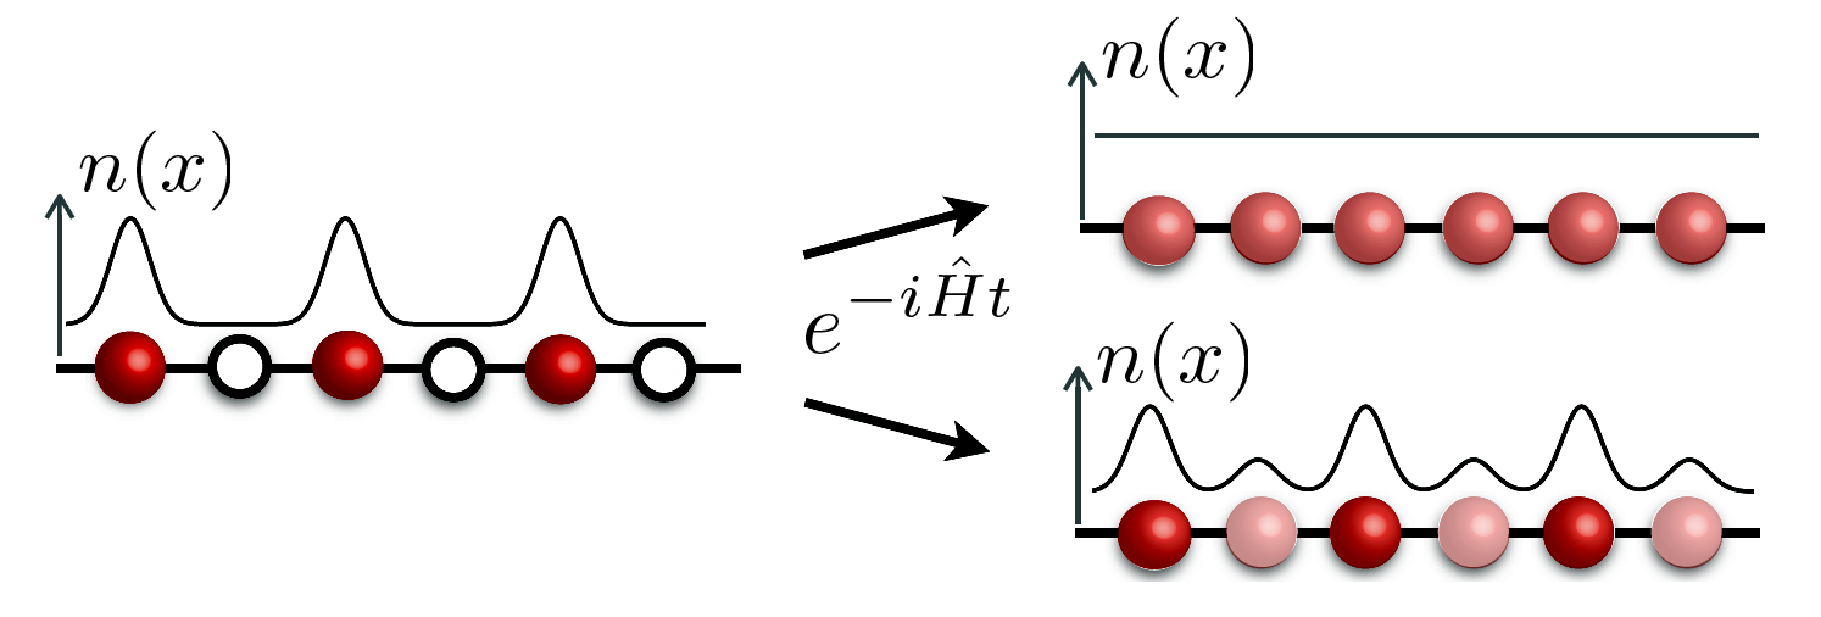
\includegraphics[width=0.95\textwidth]{abanin_thermalization_scheme.pdf}}
\caption{
Shematski prikaz razlike med unitarnim časovnim razvojem netipične začetne konfiguracije interagirajočih delcev v ergodičnem in MBL režimu, kjer je netipičnost dosežena z alternirajočo zasedenostjo mest na kristalni verigi.
 V prvem primeru sistem sčasoma relaksira proti ravnovesni enakomerni porazdelitvi delcev, medtem ko se tovrstna relaksacija v MBL fazi ne zgodi - tudi po dolgem času sistem ohrani spomin na netipičnost začetnega stanja. Slika je bila vzeta iz Ref.~\cite{abanin2018ergodicity}. 
}
\label{fig:abanin_thermalization}
\end{figure}
\end{minipage}
lokalizirane 
funkcije ne
 prispevajo k transportu v sistemu in tako preprečujejo termalizacijo. Kot sta točno pokazala Mott in Twose~\cite{doi:10.1080/00018736100101271}, povzroči v eni dimenziji ob odsotnosti meddelčnih interakcij še tako majhen nered nastop Andersonove lokalizacije in odsotnost prevodnosti. Podobno velja v dveh dimenzijah~\cite{abrahams1979scaling}, medtem ko v tridimenzionalnem primeru obstaja kritična vrednost nereda, nad katero imajo sistemi izolativne, pod njo pa prevodne lastnosti~\cite{mott1990metal}. Pri ničelni temperaturi tako spreminjanje nereda vodi do prehoda med prevodno in lokalizirano fazo. \\\\
 Čeprav je enodelčna lokalizacija zaradi omenjene  vloge dimenzionalnosti pri nastopu lokalizacijskih pojavov že sama po sebi zapletena in zanimiva, odpira vključitev meddelčnih interakcij povsem nove raziskovalne možnosti. Preplet nereda in meddelčnih interakcij odpira vprašanja o možnosti obstoja MBL pri končnih temperaturah~\cite{basko2006metal}~\cite{PhysRevB.75.155111} in o zahtevanih lastnostih meddelčnih interakcij. V zadnjih letih postaja področje vse bolj privlačno ne samo zaradi rezultatov numeričnih analiz~\cite{vznidarivc2008many}~\cite{PhysRevB.75.155111}~\cite{PhysRevA.92.041601}, temveč tudi zaradi porajajočih se možnosti eksperimentalne realizacije MBL sistemov v poskusih s hladnimi atomi~\cite{PhysRevLett.114.083002}~\cite{schreiber2015observation}~\cite{PhysRevLett.116.140401}. Nekatera izmed odprtih vprašanj s področja so naslovljena tudi v raziskovalnem delu, predstavljenem v magistrski nalogi, kjer se ukvarjam s prehodom med ergodičnim in MBL režimom v kvantnomehanskem modelu t-J~\cite{spalek2007tj}. Pri preučevanju nastopa lokalizacije me zanima vloga različnih tipov nereda, posebej primerjava med vplivom nereda, ki se sklaplja s spinskimi prostostnimi stopnjami, in nereda, ki se sklaplja s prostostnimi stopnjami nosilcev naboja. Način vpeljave obeh zvrsti nereda podrobneje razložim v nadaljnjih poglavjih ob formalni predstavitvi modela.
  \\\\Raziskovalno delo temelji na numeričnih metodah, točneje polni diagonalizaciji modelskih hamiltonk in 
  analizi tako izračunanih spektrov.  Različne spektralne lastnosti hamiltonk ergodičnih in MBL modelskih sistemov izkoriščam pri analizi na podlagi teorije naključnih matrik~\cite{d2016quantum} (ang. \emph{random matrix theory}, v nadaljevanju RMT), v okviru katere so podane teoretične napovedi~\cite{mehta2004random} za vrednosti različnih spektralnih statistik in opazljivk, s katerimi primerjam svoje izračune. Med omenjenimi statistikami sta posebej izpostavljena povprečen razmik med sosednjimi nivoji in statistika razmikov sosednjih energijskih nivojev~\cite{Atas_Distribution_PhysRevLett.110.084101}~\cite{PhysRevB.75.155111}. Slednji sta zaradi sorazmerne enostavnosti implementacije pogosto uporabljani za presojo ergodičnosti oziroma lokaliziranosti sistema. Ker vsebujeta informacije zgolj o korelacijah med najbližjimi energijskimi nivoji v spektru, podajata obnašanje modelskih sistemov na najdaljših časovnih skalah. Polnejši vpogled v dogajanje na vseh časovnih skalah sistemov dobim z izračunom spektralnega oblikovnega faktorja (ang. \emph{spectral form factor}, v nadaljevanju SFF) oziroma Fourierove transformacije dvotočkovne korelacijske funkcije energijskega spektra. Izsledke metod, ki temeljijo na statističnih lastnostih energijskih spektrov, dopolnim in primerjam z izračuni prepletenostne entropije vseh lastnih stanj modelskih hamiltonk. Znanilec nastopa MBL je v tem primeru `površinsko skaliranje' prepletenostne entropije v odvisnosti od velikosti podsistema v nasprotju s `prostorninskim skaliranjem' v ergodičnih sistemih. \\\\
  V nadaljevanju uvodnega poglavja najprej podrobneje predstavim pojav Andersonove lokalizacije v neurejenih sistemih neinteragirajočih delcev in razložim pomen različnih modelov nereda. Nato prek dodatka meddelčnih interakcij obravnavo razširim na področje MBL. V drugem poglavju predstavim tipične modelske sisteme, primerne za preučevanje nastopa MBL, in sicer Heisenbergovo verigo, Hubbardov model in model t-J, ki ima osrednjo vlogo v raziskovalnem delu, predstavljenem v tej magistrski nalogi. Poleg modelov predstavim tudi numerično implementacijo točne diagonalizacije. V tretjem poglavju predstavim statistične lastnosti hamiltonskih spektrov in vpeljem ključne pojme s področja RMT. Predstavljeni so rezultati analize sosednjih energijskih nivojev v odvisnosti od različnih tipov nereda in rezultati analize SFF. Četrto poglavje je namenjeno vpeljavi prepletenostne entropije in predstavitvi izračunov za to količino. 




%ne sme manjkati: kaj so še razlike: poleg zloma ergodičnosti in odsotnosti transporta je tu še spektralna statistika in prepletenostna entropija -> to mi študiramo. Potem lahko pride na vrsto že predstavitev vsebine po poglavjih. 
%sistem pripravljen v neravnovesnem stanju -> kaj se zgodi - > lahko termalizira, lahko pa ne; ETH ne ubogajo MBL 
%integrabilni sistemi -> MBL: vanishing transport 
\newpage
%KLJUČNE TEME: 
%MBL
%TERMALIZACIJA, EKVILIBRACIJA, VLOGA NEREDA
%
%NAVEŽI SE TUDI NA SEMINAR IN ANDERSONA
% Kaj navesti: glej: MBL and thermalization in disordered Hubbard chains (Rigol, Mondaini) - naštej, zakaj je to pomembno, od kdaj je to zanimivo in kateri članki pridejo v poštev -> 
% vloga nereda v sistemu -> vpelješ, glej Abanin => začneš z Andersonom, omembo prelomnega članka (1958), tu se lahko nanašaš na seminar. Sicer večino teksta pri seminarju pride v poštev v naslednjem podpoglavju
% v uvodu: obvezno slika Abanin (kaj je to lokalizacija, kaj je značilnost sistema, kako je s termalizacijo). Glej Nandkishore, Huse za razlago, kaj je MBL in zakaj je pomemben
% MBL represents a new frontier of quantum statistical mechanics. MBL systems fail to thermally equilibrate, so their long-time states are not captured by conventional equilibrium statistical mechanics ... 
\subsection{Andersonova lokalizacija in osnove neurejenih kvantnih sistemov}\label{anderson}
Obravnavo lokalizacijskih pojavov začnem z vpeljavo pojma Andersonove lokalizacije, ki nastopi v neurejenih sistemih neinteragirajočih delcev. Razumevanje mehanizmov, ki vodijo do lokalizacije ob odsotnosti interakcij, je namreč dobrodošla osnova za razširitev obravnave z dodatkom meddelčnih interakcij in posledično preučevanje MBL pojavov. \\\\	
Zahvaljujoč se translacijski simetriji lahko v idealno urejenih kristalnih strukturah elektronske valovne funkcije  opišemo kot prostorsko razsežne Blochove valovne funkcije. Stanja dejanskih sistemov se pogosto bistveno razlikujejo od tovrstnega idealiziranega opisa, saj je zaradi tako rekoč neizogibne prisotnosti nečistoč, defektov in vrzeli idealna kristalna urejenost v praksi le bolj ali manj dobra predpostavka. Pri tem se v razpravi o neurejenih sistemih uporabljan pojem \emph{nereda} nanaša na vsa omenjena odstopanja od idealne urejenosti.  V limiti majhnega nereda, ko se odstopanja od sicer popolne ureditve pojavijo le na nekaj mestih, so valovne funkcije sistema še vedno prostorsko razsežne in le malo odstopajo od ravnih valov. Z naraščanjem nereda se lahko njihova narava popolnoma spremeni, saj lahko nekatere  postanejo lokalizirane z eksponentno pojemajočo ovojno funkcijo, kot prikazuje Slika~\ref{fig:dif_loc_ext}.
\begin{minipage}[t]{0.57\textwidth}
\noindent 
 Elektroni z lokaliziranimi valovnimi funkcijami so znotraj sistema omejeni na končna območja in zato zanemarljivo malo vplivajo na transportne lastnosti, medtem ko elektroni zasedajoč prostorsko razsežna stanja tipično prispevajo h končnemu transportu. Posledično je sistem izolator, če pod njegovo Fermijevo energijo obstajajo zgolj lokalizirana stanja, in prevodnik, v kolikor Fermijev nivo sovpada z energijo prostorsko razsežnih stanj~\cite{kramer1993localization}. Za razlago obstoja prevodnikov in izolatorjev in razlik med njimi je torej ključno razumevanje vloge nereda pri lokalizaciji kvantnomehanskih valovnih funkcij. Poleg vpliva količine nereda in dimenzionalnosti sistema so v tem podpoglavju razloženi tudi osnovni pojmi s področja Andersonove lokalizacije. V magistrski nalogi se pojem lokalizacija nikoli ne nanaša na
\end{minipage}\hfill
\begin{minipage}[t]{0.4\textwidth}
\begin{figure}[H]
\centering{
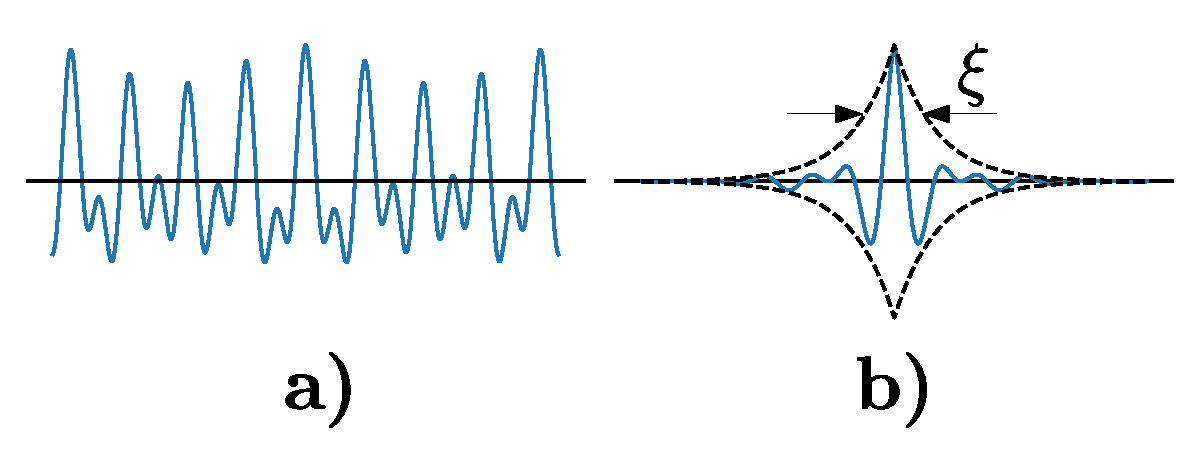
\includegraphics[width=0.85\textwidth]{diff_loc_ext_mod.pdf}}
\caption{Teorija Andersonove lokalizacije napove možnost lokalizacije kvantnomehanskih stanj zaradi naključnih potencialov. \textbf{a)} Primer razsežnega stanja. \textbf{b)} Lokalizirano stanje, katerega ovojnica eksponentno pojema z razdaljo od neke točke v prostoru. $\xi$ je lokalizacijska dolžina. 
}
\label{fig:dif_loc_ext}
\end{figure}
\end{minipage}
 t.i. Mottovo lokalizacijo, ki je posledica močnih odbojnih medelektronskih interakcij in je v nalogi ne obravnavam. \\\\
Možnost lokalizacije elektronskih valovnih funkcij ob prisotnosti dovolj močnega potencialnega nereda je leta 1958 prvi napovedal P.W. Anderson~\cite{anderson1958absence}. Medtem ko sta limitna primera šibkega in močnega nereda intuitivno razmeroma lahko predstavljiva, je bilo vprašanje o obnašanju sistemov v vmesnem režimu, posebej v dveh dimenzijah, dolgo časa odprto. Mott in Twose sta za enodimenzionalne sisteme eksaktno dokazala~\cite{doi:10.1080/00018736100101271} nastop lokalizacije ob prisotnosti vsakršnega končnega nereda, enak rezultat pa  v termodinamski limiti neskončnih sistemov velja tudi v dveh dimenzijah~\cite{abrahams1979scaling}. Kot je leta 1968 pokazal Mott, obstaja v treh dimenzijah kritična energija $E_c$ oziroma \emph{rob mobilnosti}~\cite{mott1990metal}, ki loči lokalizirana od razsežnih stanj. Energija prvih je manjša, drugih pa večja od kritične energije $E_c$. Obstoj roba mobilnosti danes označuje nastop z neredom vzbujenega faznega prehoda med kovino in izolatorjem. Leta 1977, manj kot 20 let po objavi prelomnega članka, je bila Andersonu za njegovo delo podeljena Nobelova nagrada za fiziko~\cite{anderson1978local}.
 \subsubsection{Opis prevodnosti pred teorijo lokalizacije in po njej}  
 Lokalizacija kvantnomehanskih delcev v naključnih potencialih je zanimiv statističnofizikalni pojav. Pred razvojem teorije Andersonove lokalizacije je bila elektronska prevodnost tipično opisovana v okviru kvantnomehanske različice Drudejevega modela. Pri slednjem privzamemo sorazmernost prevodnosti s \emph{povprečno prosto potjo} $l$, torej razdaljo, ki jo delec v snovi prepotuje pred trkom z nečistočo. V kvantnomehanskem smislu to pomeni, da se valovni paketi pri propagaciji vzdolž neurejenega medija na naključnem potencialu v povprečju sipajo po prepotovani razdalji $l$. Čeprav zaradi sipanja na naključnem potencialu valovni paketi nimajo več ostro določenega valovnega vektorja, ostanejo valovne funkcije sipanju navkljub prostorsko razsežne. Na daljših razdaljah je tovrstna propagacija skozi medij difuzivna, povečanje količine nereda v sistemu pa vodi do zmanjšanja povprečne proste poti. Zaradi predpostavke sorazmernosti med prevodnostjo in povprečno prosto potjo Drudejev model pri nobenem končnem neredu ne napove ničelne prevodnosti. Napovedi modela so bile v nasprotju s presenetljivo dolgimi relaksacijskimi časi elektronskih spinov, izmerjenimi v poskusih z dopiranimi polprevodniki, ki jim je v petdesetih letih v Bellovih laboratorijih prisostvoval Anderson~\cite{lagendijk2009fifty}~\cite{anderson1978local}. V nasprotju z Drudejevim modelom rezultate uspešno razloži model, v katerem valovne funkcije pri dovolj močnem neredu postanejo lokalizirane z eksponentno pojemajočo ovojnico, $\left|\psi\left(\textbf{r}\right)\right|   \sim \exp\left(\left|\textbf{r}- \textbf{r}_0\right|\right/\xi)$, kjer je $\xi$ \emph{lokalizacijska dolžina}. V kolikor so vse valovne funkcije lokalizirane, se dizufivna propagacija v neurejenem mediju ne samo upočasni, temveč popolnoma ustavi - delci postanejo ujeti, prevodnost pa pade na ničelno vrednost~\cite{wolfle2010self}. Presenetljiv rezultat je možno razložiti preko obravnave večkratne interference valovnih komponent, sipanih na naključno porazdeljenih sipalcih - lokalizacija je namreč v svojem bistvu interferenčni pojav. 
 \subsubsection{Ojačano povratno sipanje}
 Pomen interferenčnih pojavov pri nastopu Andersonove lokalizacije je vsaj intuitivno najlažje razložiti z uporabo osnovnih načel valovne mehanike. Privzemimo limito šibkega nereda in obravnavajmo delec, ki se v neurejenem mediju propagira med točkama $\textbf{r}_0$ in $\textbf{r}_1$. Za izračun verjetnosti delčevega prihoda v točko $\textbf{r}_1$ moramo sešteti vse kompleksne verjetnostne amplitude različnih poti med točkama in izračunati kvadrat absolutne vrednosti končne vsote. Verjetnost na koncu podajata vsota kvadratov posameznih verjetnostnih amplitud ter vsota mešanih, interferenčnih členov. Prva ustreza klasičnemu nekoherentnemu prispevku, drugo pa lahko v večini primerov upravičeno zanemarimo zaradi predpostavke naključne porazdelitve faz interferenčnih členov v neurejenem mediju. Z neupoštevanjem interferenčnih členov dobimo namesto napovedi lokalizacije Drudejev opis prevodnosti v neurejenih sistemih, torej očitno obstajajo primeri, v katerih interfenčnih členov ne smemo zanemariti. \\\\
 \begin{minipage}[t]{0.58\textwidth}
\noindent  
Naj bo delec uvodoma v točki $\mathbf{r}_0$ in naj bo $A_1$ verjetnostna amplituda za proces, v katerem se delec vzdolž neke poti $C_1$ vrne v izhodiščno točko, $A_2$ pa naj bo amplituda povratka v izhodiščno točko vzdolž neke druge poti $C_2$, kot prikazuje Slika~\ref{fig:paths}.
Skupno verjetnost povratka podaja zveza 
\begin{equation}
w=|A_1 + A_2|^2=w_\mathrm{cl} + w_\mathrm{int},
\end{equation}
kjer je $w_\mathrm{cl}=|A_1|^2 + |A_2|^2$ in $w_\mathrm{int}=2\Re\left(A_1^*A_2\right)$ \cite{wolfle2010self}. Za različni poti $C_1$ in $C_2$ se interferenčni členi v povprečju izničijo in je njihovo neupoštevanje upravičeno. Drugače je v posebnem primeru, ko je  $A_2=A_r$ verjetnostna amplituda za proces, v katerem povratek poteka vzdolž poti $C_1$, vendar v obratni smeri. V kolikor je sistem simetričen na obrat časa, $A_1=A_r$, potem s pravilnim upoštevanjem interferenčnih  členov izračunamo dvakrat večjo verjetnost povratka kot v klasičnem primeru: 
\end{minipage}\hfill
\begin{minipage}[t]{0.39\textwidth}
\begin{figure}[H]
\centering{
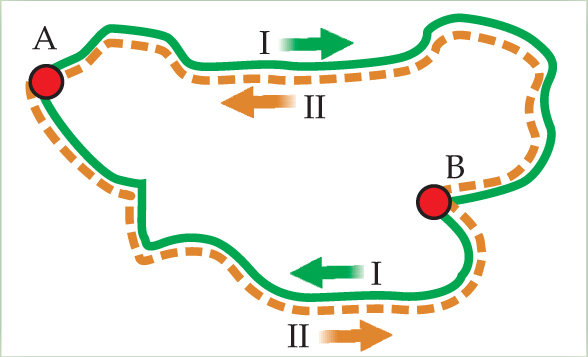
\includegraphics[width=0.9\textwidth]{interference.jpg}}
\caption{Shematski prikaz valovnega paketa, ki se preko poti I skozi točko B vrne v izhodično točko A. Pot II je enaka poti I, le da je obrnjena v času. Slika je bila vzeta iz \cite{lagendijk2009fifty}.}
\label{fig:paths} 
\end{figure}
\end{minipage}
\begin{equation}
w=4\left|A_1\right|^2=2w_\mathrm{cl}.
\end{equation}
Zaradi konstruktivne interference poti z njeno v času obrnjeno ustreznico je torej pri sipalnem dogodku verjetnost za povratno sipanje v izhodiščno točko večja od verjetnosti vseh preostalih izidov dogodka. Pojav imenovan \emph{ojačano povratno sipanje} zmanjša transmitivnost medija in posledično zmanjša tudi njegovo prevodnost. 
\subsubsection{Skalirna teorija lokalizacije}
Lokalizacija v neurejenih sistemih je netrivialno odvisna od njihove dimenzionalnosti. Medtem ko v eni dimenziji vsakršnen končni nered povzroči lokalizacijo vseh valovnih funkcij, obstaja v treh dimenzijah kritična vrednost nereda, nad katero so vsa stanja lokalizirana, za podkritične vrednosti nereda pa v sistemu soobstajajo razsežna in lokalizirana stanja. Medtem ko za dvodimenzionalne sisteme~\cite{kramer1993localization} rigorozen dokaz ne obstaja se zdi, da so v termodinamski limiti neskončnega sistema vse valovne funkcije lokalizirane pri vsakršni končni vrednosti nereda, podobno kot v enodimenzionalnem primeru. Za razliko od neskončnih sistemov lahko končni dvodimenzionalni sistemi kažejo prevodne lastnosti. \\\\ 
Opisana zapletena vloga dimenzionalnosti pri nastopu lokalizacijskih pojavov je danes pogosto razložena v okviru \emph{skalirne teorije} lokalizacije, ki so jo leta 1979 razvili Abrahams, Anderson, Licciardello in Ramakrishnan~\cite{abrahams1979scaling}. Navkljub svoji preprostosti in fenomenološkemu pristopu teorija pravilno napove glavne lastnosti lokalizacije v različnih dimenzijah in tako ob odsotnosti rigoroznega teoretičnega modela ponuja dragocen uvid v značilnosti lokalizacijskih pojavov. Skalirna teorija opisuje Andersonovo lokalizacijo v jeziku kritičnih fenomenov zveznih kvantnih faznih prehodov. Slednji nastopijo pri ničelni temperaturi in jih namesto temperature vodi spreminjanje nekega drugega parametra - v primeru lokalizacijskih pojavov je to količina nereda v sistemu. Ker gre za teorijo faznih prehodov, skalirna teorija za različne količine napove skalirne zakone. Tu bo na kratko predstavljena le skalirna zveza za specifično prevodnost.\\\\
Pred nadaljevanjem se spomnimo, da sta v tridimenzionalnem ohmskem prevodniku prevodnost $g$ in specifična prevodnost $\sigma$ povezani z zvezo $g=\sigma\frac{S}{L}.$ Pri tem je $S$ prečni presek prevodnika in $L$ njegova dolžina. Pri skalirni teoriji v splošnem obravnavamo odvisnost prevodnosti $d$-dimenzionalne hiperkocke od dolžine njene stranice $L$, zato uvedemo logaritemski odvod $\beta$ kot 
\begin{equation}\label{eq:beta_log}
\beta=\frac{\dd \log g}{\\d \log L}.
\end{equation}
Teorija privzame eksplicitno odvisnost $\beta$ zgolj od $g$, ne pa tudi od energije, nereda ali dolžine stranice $L$. Kvalitativno obnašanje količine $\beta$ določata znani asimptotski limiti majhne in velike prevodnosti, medtem ko so vmesne vrednosti določene z interpolacijo ob predpostavki, da je $\beta$ zvezna in monotono naraščajoča funkcija. \\\\
\begin{minipage}[t]{0.54\textwidth}
Iz En. \eqref{eq:beta_log} je očitno naraščanje $g$ z velikostjo sistema v primeru $\beta>0$, kar označuje kovinski oziroma preveden značaj, v katerem velja dobro poznana klasična zveza med prevodnostjo in specifično prevodnostjo,
\begin{equation}\label{eq:g_prevodnik}
g(L)=\sigma\frac{L^{d-1}}{L}=\sigma L^{d-2}.
\end{equation}
Zgoraj zapisana zveza za ohmski prevodnik je le poseben primer En.~\eqref{eq:g_prevodnik}, ki nam v prevodnem območju da zvezo $\beta=d-2$. Posledično je količina $\beta$ pozitivna le za tridimenzionalne prevodnike, ničelna v dveh in negativna v eni dimenziji. V nasprotni, torej lokalizirani limiti, $g$ pojema eksponentno z velikostjo sistema, $g\propto \exp(-L)$ in $\beta<0$. Dejanska funkcijska odvisnost je v tem režimu podana z zvezo 
\begin{equation}
\beta=\frac{\dd \log g}{\dd L}\frac{\dd L}{\dd \log L}=\log g
\end{equation}
\end{minipage}\hfill
\begin{minipage}[t]{0.43\textwidth}
\begin{figure}[H]
\centering{
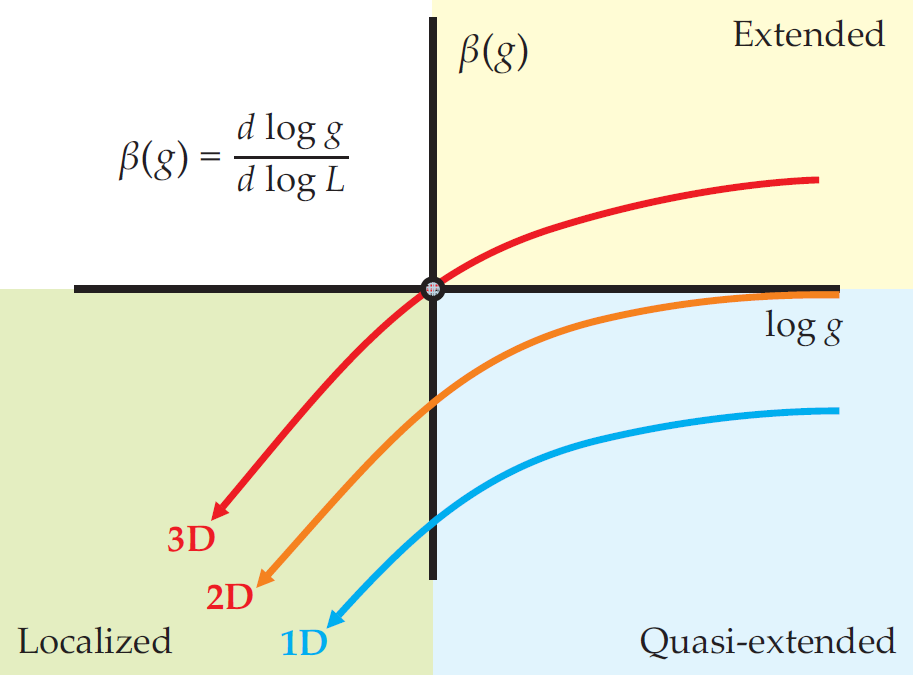
\includegraphics[width=0.8\textwidth]{beta_diagram.png}}
\caption{Skalirna teorija napove fazni prehod med prevodnikom in izolatorjem le v treh dimenzijah, saj v nižjedimenzionalnih sistemih prevodnost z velikostjo sistemov vselej pada. Slika je bila vzeta iz~\cite{lagendijk2009fifty}.}
\label{fig:scalingtheory} 
\end{figure}
\end{minipage}\\\\
Prehod med izolatorjem in prevodnikom se zgodi v kritični točki $\beta(g_c)=0$. To je možno zgolj v treh dimenzijah, kjer $\beta$ zavzame tako negativne kot pozitivne vrednosti. V nižjih dimenzijah prevodnost z naraščanjem velikosti sistema vedno pada in tako kritična točka ni nikoli dosežena. 
\subsubsection{Modeli nereda}
V tem podpoglavju predstavim različne modele nereda v kvantnomehanskih sistemih. Podana je razlaga uvedbe nereda v idealno urejene kristalne sisteme, kot najpogosteje uporabljan model neurejenega sistema neinteragirajočih delcev pa je podrobneje predstavljen Andersonov model. \\\\
Opis translacijsko invariantnih sistemov je zaradi njihove translacijske simetrije razmeroma enostaven. Enoelektronske valovne funkcije so v teh sistemih Blochovega tipa, posledično so elektroni prosto gibljivi. V večini dejanskih sistemov je idealna translacijska simetrija zlomljena zaradi prisotnosti nereda, ki lahko bistveno vpliva na fizikalne lastnosti sistemov. V primeru nizke koncentracije defektov lahko pri opisu neurejenih sistemov kot izhodišče uporabimo koncepte, veljavne v translacijsko invariantnih sistemih. Na drugi strani velika koncentracija defektov terja popolno opustitev predpostavke translacijske simetrije in uporabo novih pristopov. \\\\
\begin{minipage}[t]{0.54\textwidth}
Kot prikazuje Slika~\ref{fig:disorder_scheme}, lahko različne modele nereda dobimo s takšno ali drugačno deformacijo idealne kristalne strukture. Modele za opis \emph{strukturno neurejenih} sistemov, kot so npr. amorfni polprevodniki,  dobimo z naključnimi premiki delcev z mest na urejeni kristalni rešetki. Enodelčno hamiltonko takšnega sistema podaja 
\begin{equation}\label{eq:cont_ham}
H=\frac{\hat{p}^2}{2m} + \sum\limits_{j=1}^N V_j(\textbf{r}- \textbf{R}_j), 
\end{equation}
kjer je $\hat{p}$ operator gibalne količine, $m$ efektivna masa delca, $V_j$ pa potencialna energija atoma na mestu $\textbf{R}_j$. Nered vpeljemo z naključno izbiro potencialnih energij in položajev $\textbf{R}_j$, kjer vrednosti žrebamo v skladu z nekima izbranima normaliziranima verjetnostnima porazdelitvama. \\\\
\emph{Kompozicijsko neurejene} sisteme, ki so tudi osrednji predmet preučevanja v magistrski nalogi, najpogosteje opiše hamiltonka v približku tesne vezi na diskretni mreži:
\end{minipage}\hfill
\begin{minipage}[t]{0.43\textwidth}
\begin{figure}[H]
\centering{
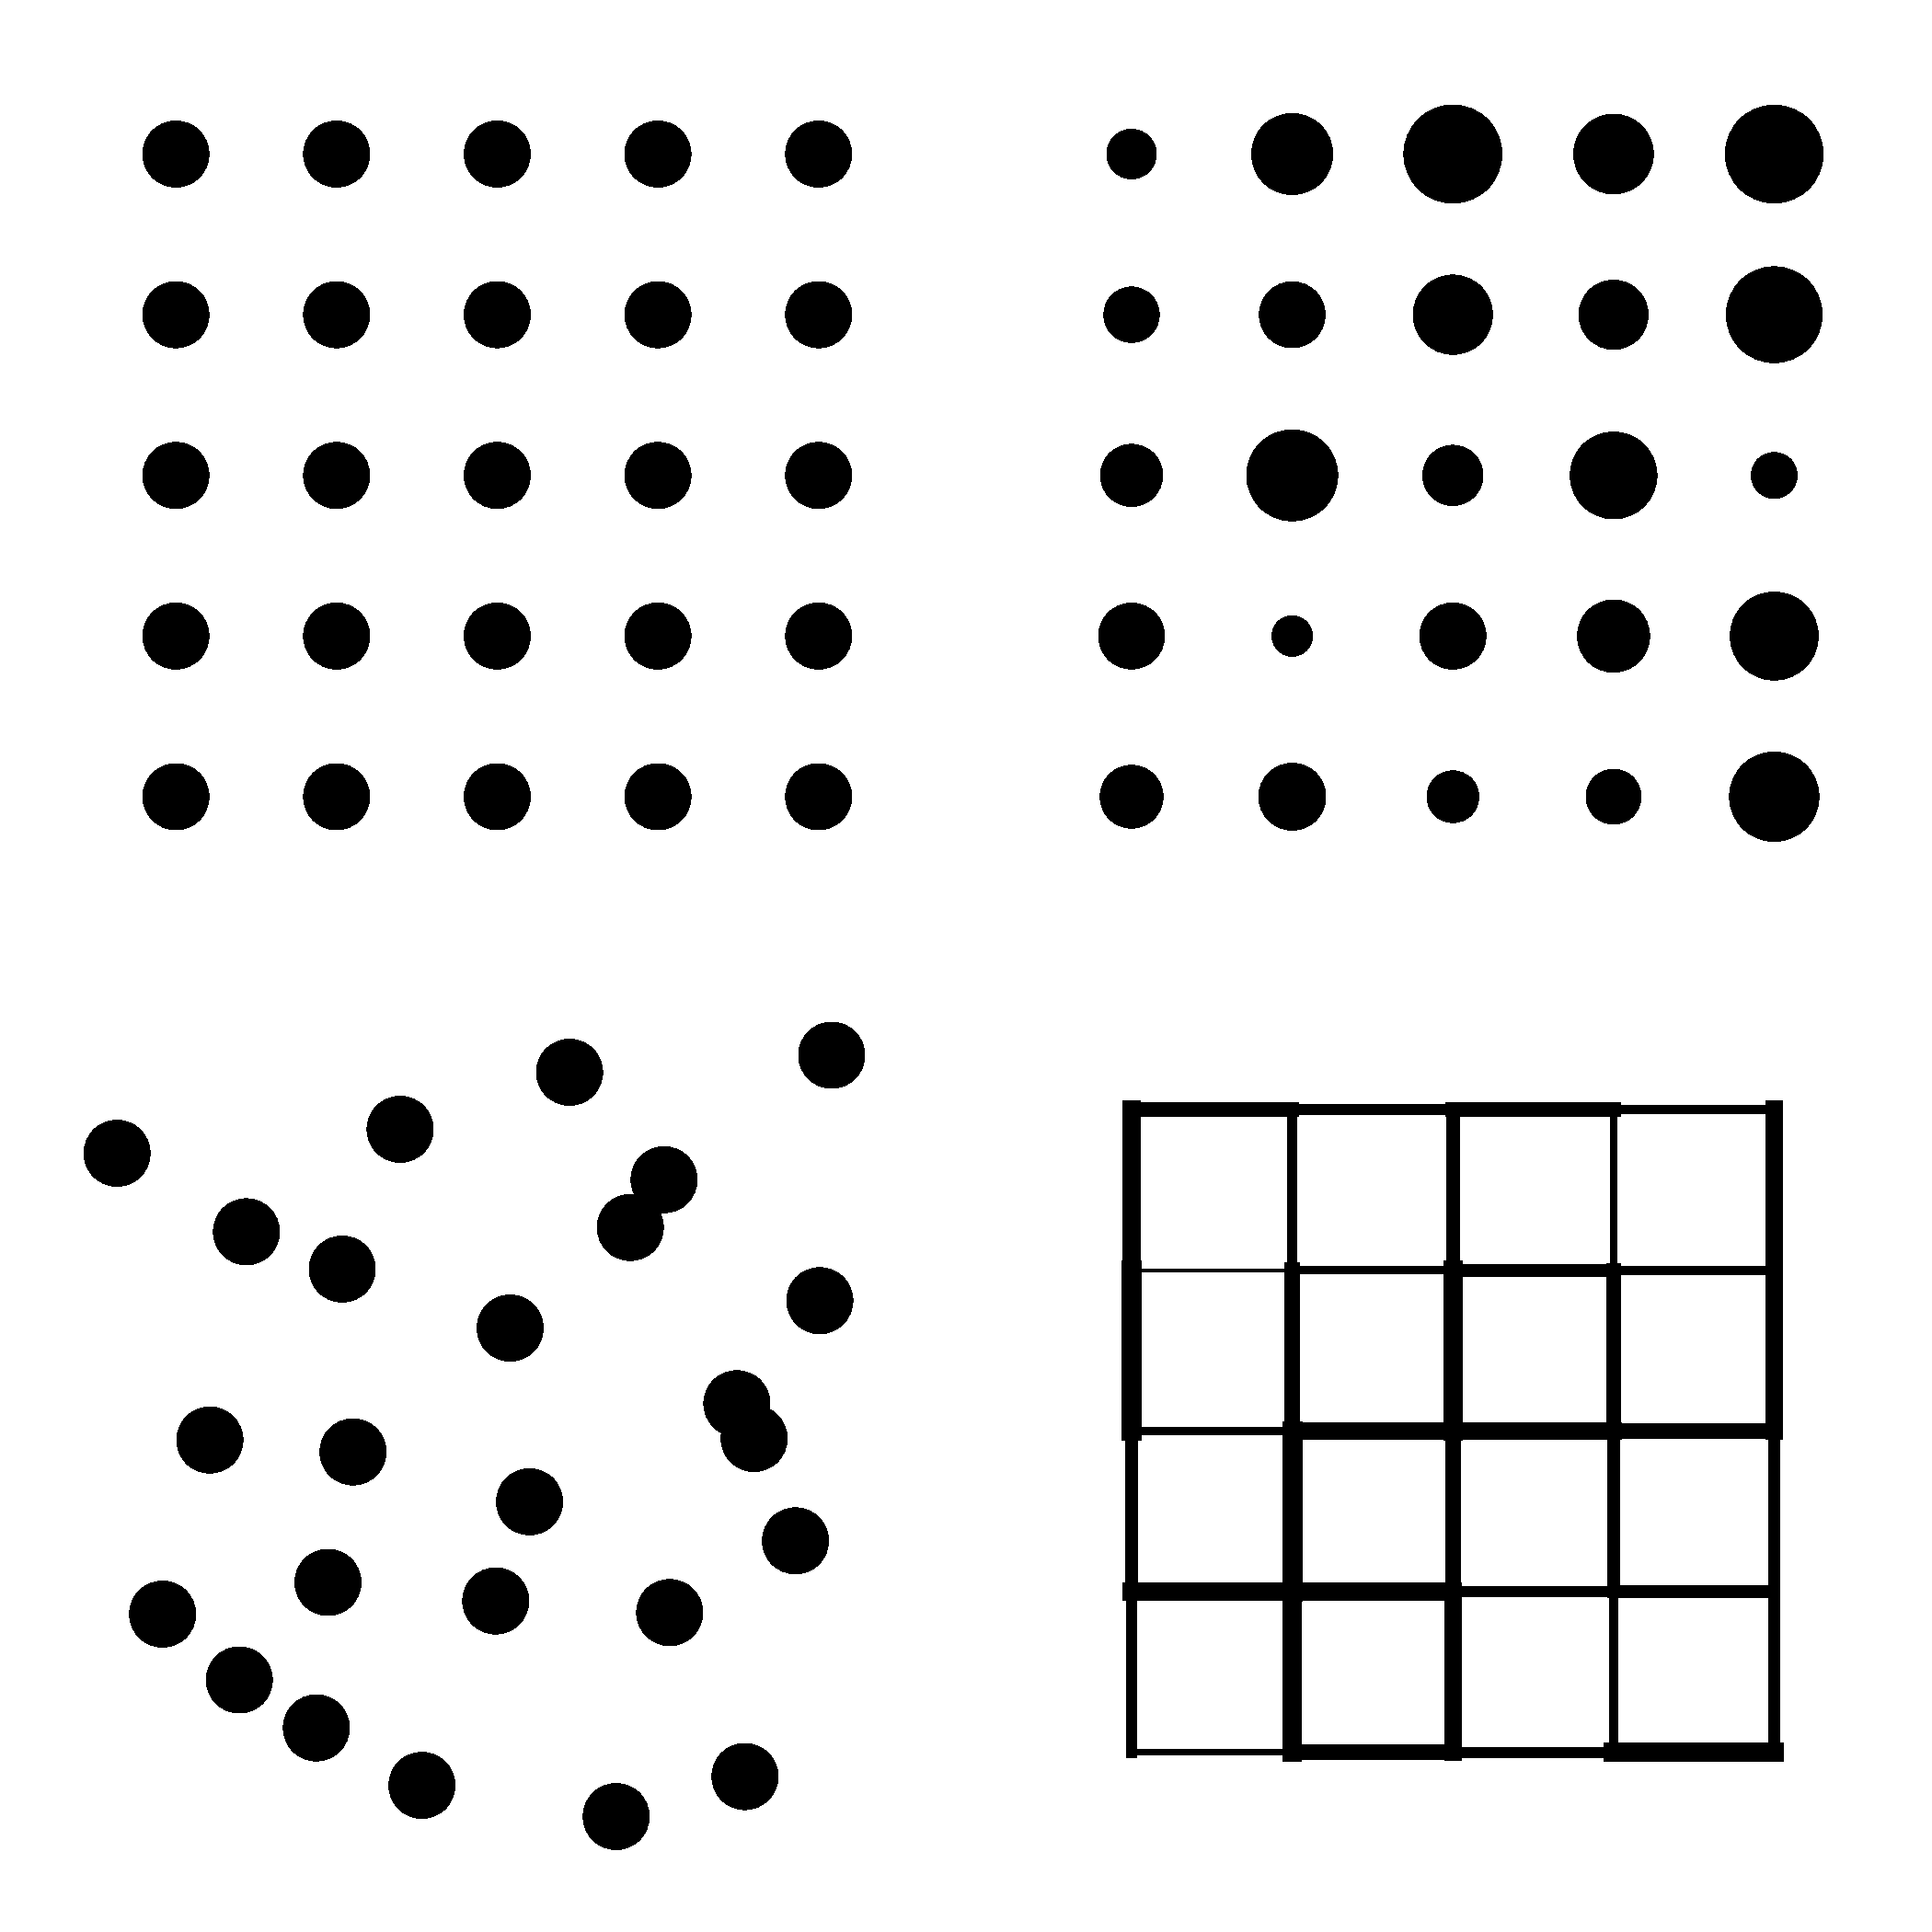
\includegraphics[width=0.8\textwidth]{disorder_scheme.pdf}}
\caption{Od leve proti desni in od zgoraj navzdol so razzvrščeni shematski prikazi idealnega kristala, kompozicijsko neurejenega sistema, strukturno neurejenega sistema in sistema s kinetičnim neredom.  }
\label{fig:disorder_scheme} 
\end{figure}
\end{minipage}\\\\
\begin{equation}\label{eq:disc_ham}
H=\sum\limits_{j\nu}U_{j\nu}c^\dagger_{j\nu}c_{j\nu} + \sum\limits_{j\nu, k\mu} t_{j\nu, k\mu} c^\dagger_{j,\nu}c_{k\mu}.
\end{equation}
Tu so $c^\dagger_{j\nu}, c_{j\nu}$ fermionski kreacijski in anihilacijski operatorji za mesto $j$ v kristalni rešetki in stanje $\nu$. Z $U_{j\nu}$ so v diagonalnem delu označene potencialne energije stanj na danih mestih v kristalni rešetki, medtem ko izvendiagonalni matrični elementi $t_{j\nu, k\mu}$ ustrezajo tunelskim prehodom med stanji na različnih mestih na mreži. Nered je vpeljan preko naključnih vrednosti potencialnih členov $U_{j\nu}$ ali skakalnih členov $t_{j\nu, k\mu}$, kjer pri žrebanju vrednosti ponovno privzamemo neko verjetnostno porazdelitev. V nasprotju z modelom, ki ga podaja En.~\eqref{eq:cont_ham}, tu ni strukturnega nereda, saj so mesta v kristalni rešetki dobro definirana in sovpadajo z mesti urejene kristalne mreže.  \\\\
\begin{minipage}[t]{0.54\textwidth}
\noindent
\textbf{Andersonov model}~\cite{anderson1958absence} je poseben primer modela, ki ga podaja En.~\eqref{eq:disc_ham}. Dobimo ga z upoštevanjem predpostavk izključno diagonalnega prispevka k neredu, skakanja elektronov zgolj med najbližjimi sosedi s konstantno hitrostjo tuneliranja $t$ in prisotnostjo le ene orbitale, $\nu=1$. Naključne potencialne energije $V_j$ so porazdeljene enakomerno na intervalu $\left[-W,W\right]$ v skladu s porazdelitvijo
\begin{equation}\label{eq:and_prob}
p(V_j)= \frac{1}{2W}\Theta \left(W - \abs{V_j} \right),
\end{equation}
kjer je $W$ \emph{parameter moči nereda}. Hamiltonka Andersonovega modela se tako zapiše kot 
\begin{equation}\label{eq:Anderson_ham}
H=\sum\limits_j U_j c^\dagger_jc_j + t\sum\limits_{\mathrm{n. s.}}\left(c^\dagger_i c_j + \mathrm{h.c.}\right).
\end{equation}\\\\

\end{minipage}\hfill
\begin{minipage}[t]{0.43\textwidth}
\begin{figure}[H]
\centering{
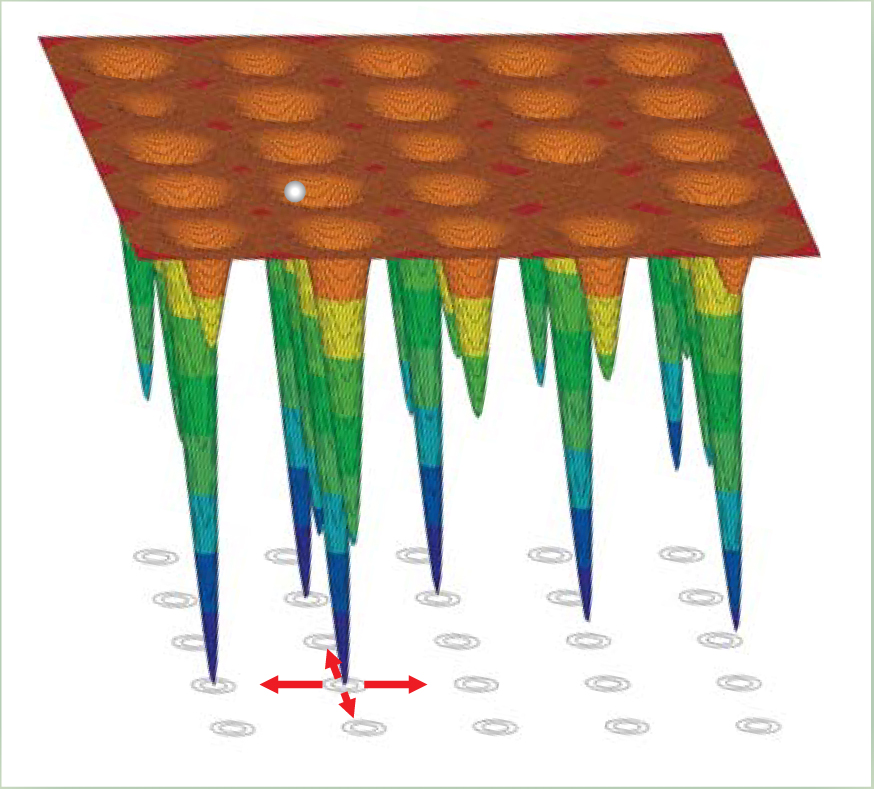
\includegraphics[width=0.65\textwidth]{hopping_picture_50years.jpg}}
\caption{Shematski prikaz Andersonovega modela v dveh dimenzijah. Elektron lahko na urejeni kristalni mreži skače med sosednjimi mesti, ki imajo naključno porazdeljene potencialne energije. Slika je bila vzeta iz~\cite{lagendijk2009fifty}.  }
\label{fig:hopping_picture} 
\end{figure}
\end{minipage}\\\\
\noindent 
\begin{minipage}[t]{0.56\textwidth} 
Ob odsotnosti nereda je Andersonova hamiltonka običajna hamiltonka v približku tesne vezi, ki opisuje urejeno mrežo enakih potencialnih jam, ki je prikazana na shemi \textbf{a)} na Sliki~\ref{fig:band_structure}.  V tem primeru jo diagonaliziramo z uporabo Fourierove transformacije in pri izračunu spektra dobimo energijski pas širine $2zt$, kjer je $z$ koordinacijsko število kristalne rešetke. Hamiltonko Andersonovega modela dobimo z naključnim spreminjanjem globin posameznih potencialnih jam za vrednosti $U_j$, ki so porazdeljene v skladu s porazdelitvijo, ki jo podaja En.~\eqref{eq:and_prob}. Kot prikazuje shema \textbf{b)} na Sliki~\ref{fig:band_structure}, dodatek nereda razširi energijski pas in odpravi singularnosti v gostoti stanj, ki so sicer značilne za sisteme z redom dolgega dosega. \\\\
V limiti zelo močnega nereda, kjer velikost parametra nereda $W$ primerjamo s hitrostjo tuneliranja $t$, lahko privzamemo, da potencialni člen v En.~\eqref{eq:Anderson_ham} močno prevlada nad izvendiagonalnim skakalnim členom in tako povzroči lokalizacijo valovnih funkcij. V okviru perturbacijske teorije lahko lastne funkcije hamiltonke opišemo kot vezana stanja ali orbitale, ki postanejo lokalizirane zaradi velikih fluktuacij naključnega potenciala. V prvem približku so energije tovrstnih enoelektronskih stanj določene kar z globinami naključnih potencialnih jam, zato se energije stanj z velikim prostorskim prekrivanjem tipično močno razlikujejo. Na drugi strani so stanja s podobnimi energijami v prostoru oddaljena in se le malo prekrivajo. Ker stanja ne v enem ne v drugem primeru ne morejo medsebojno hibridizirati, ostanejo v primeru dovolj močnega nereda lokalizirana. \\\\
V treh dimenzijah za podkritične vrednosti nereda, $W<W_c$, v sistemu obstajajo tako lokalizirana kot razsežna stanja. V odsotnosti nereda so lastne funkcije Andersonove hamiltonke razsežna stanja Blochovega tipa. Uvedba majhnega nereda, ki ustreza majhnim vrednosti $W$, povzroči šibke naključne fluktuacije potenciala, ki vplivajo zgolj na stanja v bližini robov pasu, medtem ko ostanejo stanja v okolici sredine pasu bolj ali manj nespremenjena. Majhne fluktuacije potenciala namreč povzročijo nastanek plitkih \emph{naključnih} potencialnih jam, 
\end{minipage}\hfill
\begin{minipage}[t]{0.42\textwidth} 
\begin{figure}[H]
\centering{
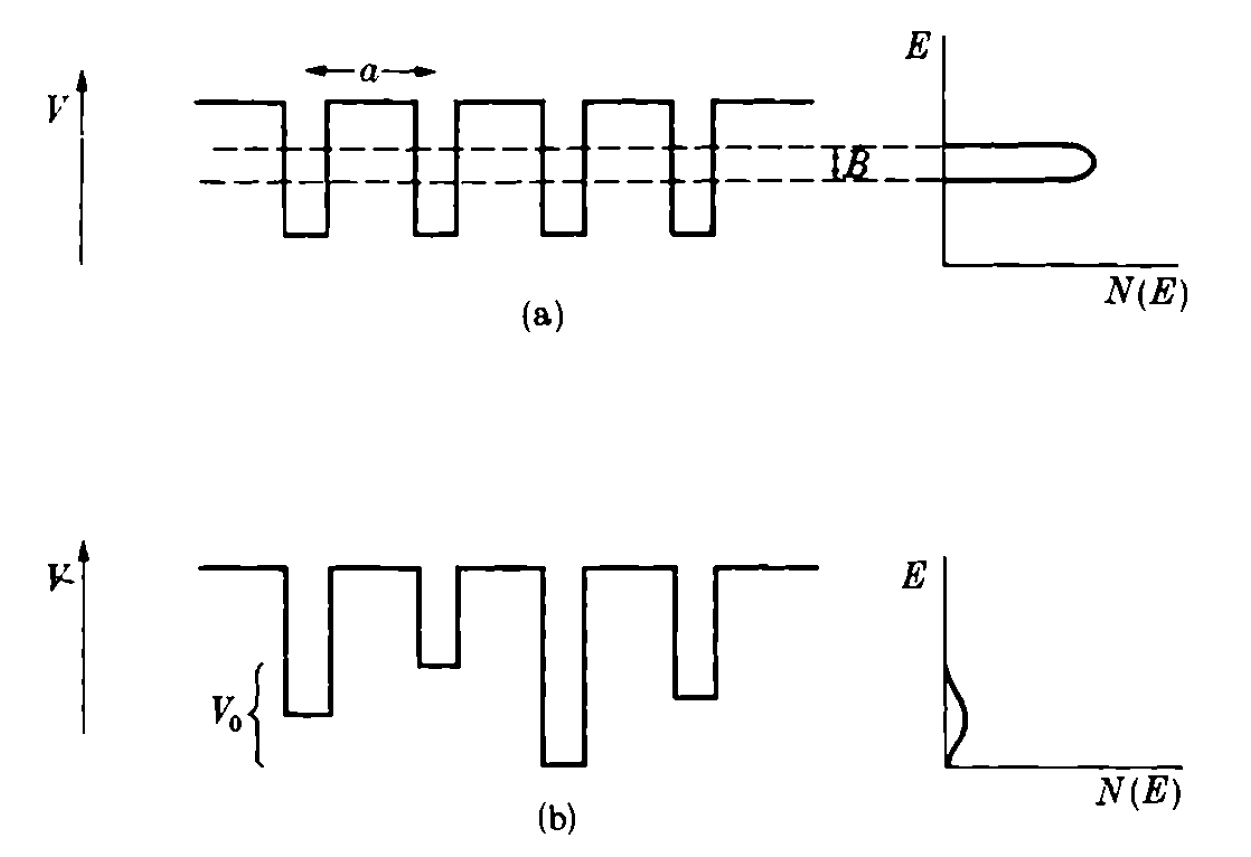
\includegraphics[width=1\textwidth]{bands.png}}
\caption{\textbf{a)} Shematski prikaz potencialnih jam za hamiltonko v približku tesne vezi ob odsotnosti nereda. \textbf{b)} Potencialne jame v Andersonovem modelu z naključnim potencialom. Na desni sta v obeh primerih shematsko prikazani gostoti stanj v treh dimenzijah. Uvedba nereda razširi pas in odpravi singularnosti gostote stanj. Slika je bila vzeta iz~\cite{mott2012electronic}.}
\label{fig:band_structure} 
\end{figure}
\begin{figure}[H]
\centering{
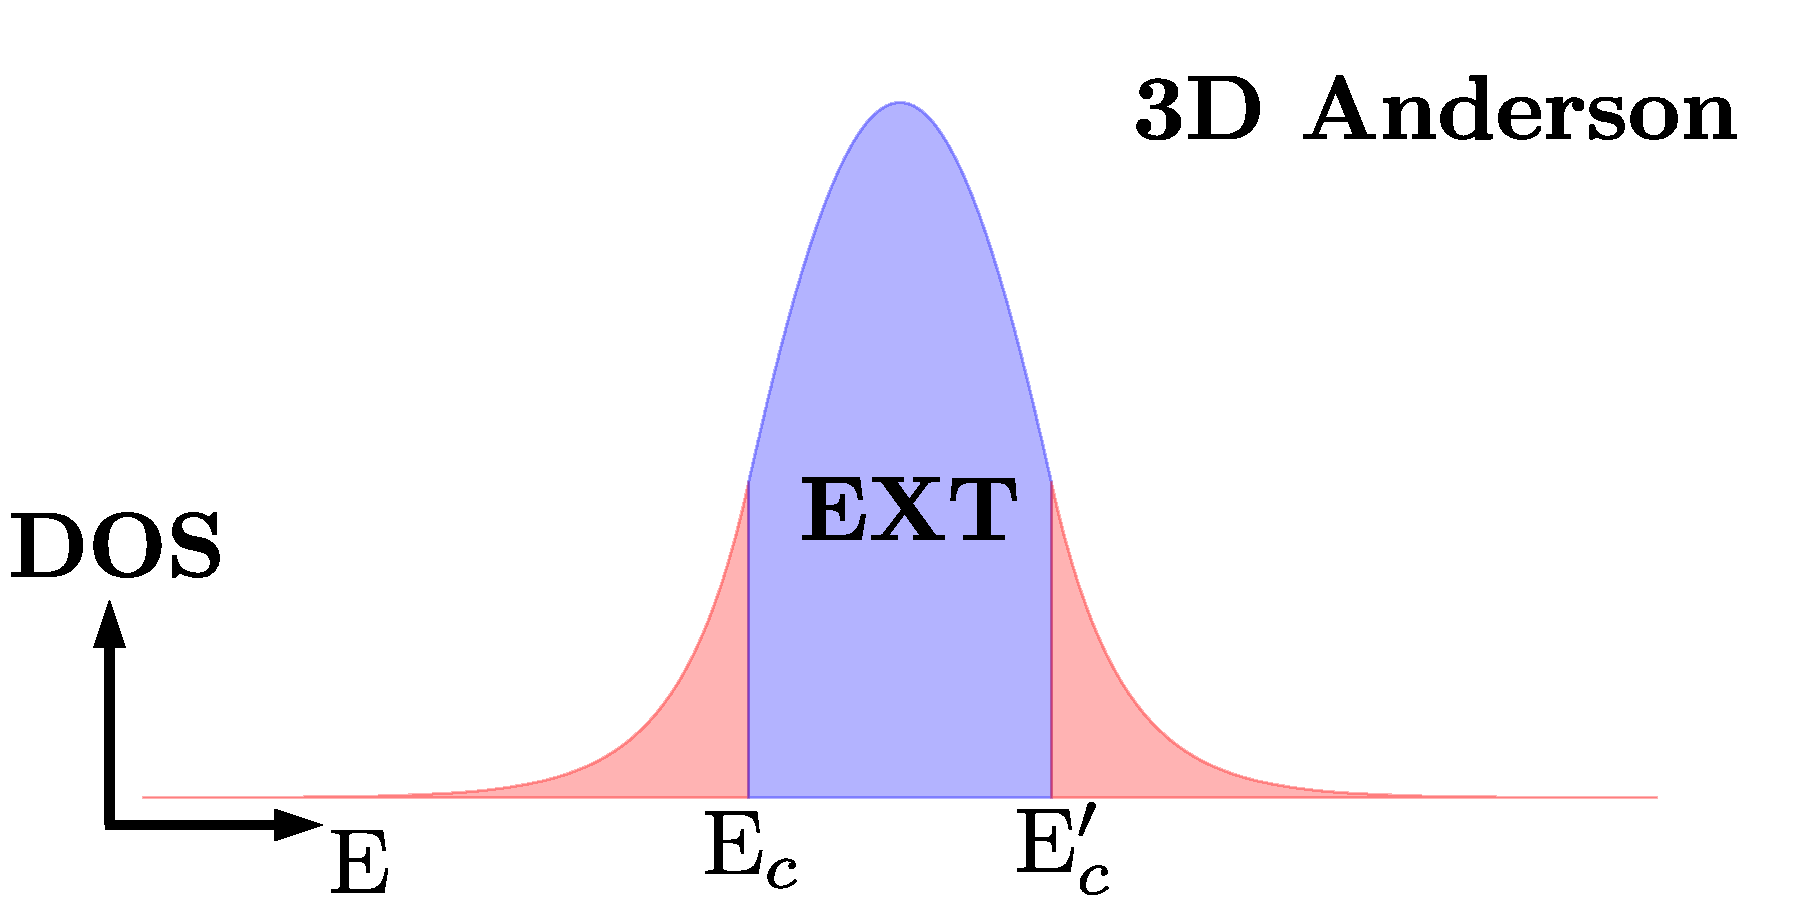
\includegraphics[width=1\textwidth]{mobility_edge_DOS_modified.pdf}}
\caption{Shematski prikaz tipične gostote stanj v odvisnosti od energije za tridimenzionalni Andersenov model za neko podkritično vrednost nereda, $W<W_c$. Stanja v robovih pasu (ki sta obarvana rdeče) so lokalizirana, medtem ko so stanja v sredini pasu (ki je obarvana modro) razsežna. $E_c$ in $E_c'$ označujeta roba mobilnosti, \textbf{EXT} pa razsežna stanja. }
\label{fig:mob_edge_DOS} 
\end{figure}
% \begin{figure}[H]
% \centering{
% 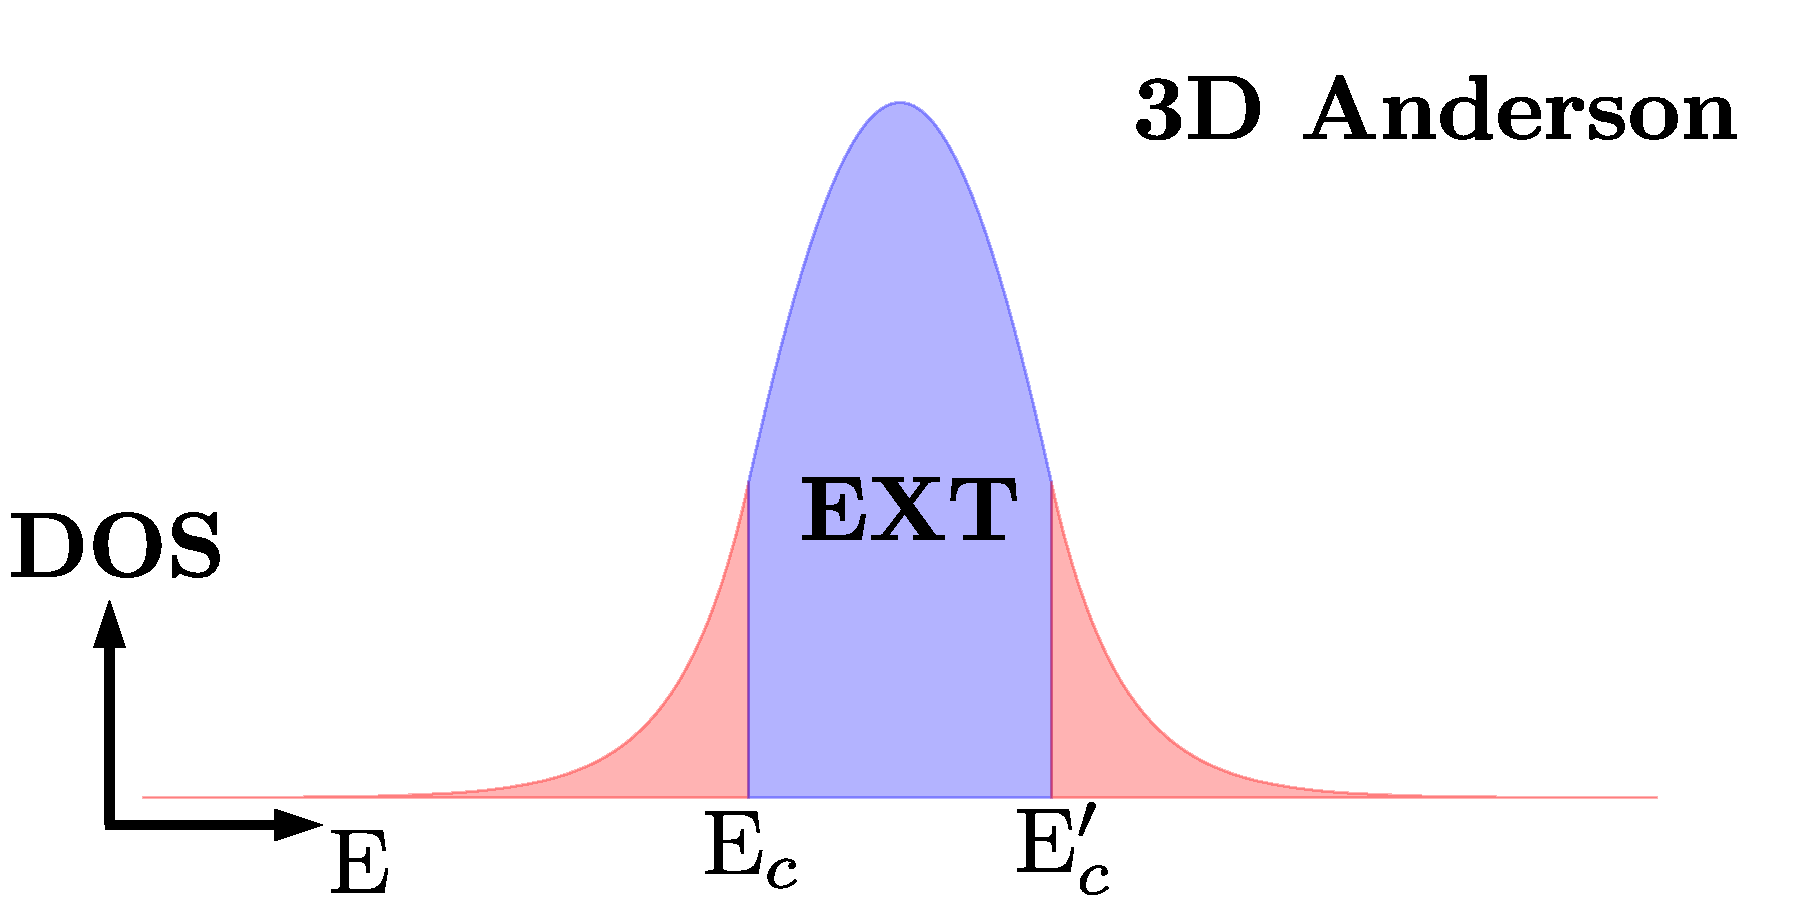
\includegraphics[width=0.95\textwidth]{mobility_edge_DOS_modified.pdf}}
% \caption{A schematic of a typical density of states (DOS) distribution with respect to energy for a three-dimensional Anderson model for some intermediate disorder $W<W_c$. States in the band tails (coloured red) are localized while those in the middle (coloured blue) are extended. }
% \label{fig:DOS} 
% \end{figure}
\end{minipage}
ki lahko lokalizirajo le nizkoenergijska lastna stanja hamiltonke. S povečevanjem parametra nereda amplituda potencialnih fluktuacij narašča, kar posledično vodi do lokalizacije stanj z višjo energijo. Lokalizirana in razsežna stanja ne morejo soobstajati pri istih energijah, saj bi v tem primeru lokalizirana stanja zaradi znatnega prekrivalnega integrala in ujemajočih se energij z razsežnimi stanji tvorila hibridizirana stanja in tako postala razsežna. Energije lokaliziranih in razsežnih stanj v splošnem loči kritična energija $E_c$ oziroma rob mobilnosti. Ker je Andersonova hamiltonka simetrična na zamenjavo delcev in vrzeli ima Andersonov model kar dva mobilnostna roba $E_c$ in $E_c'$. Kot prikazuje Slika~\ref{fig:mob_edge_DOS}, nastopata simetrično glede na središče pasu, ki se mu približujeta z naraščanjem parametra $W$. Polna lokalizacija vseh valovnih funkcij nastopi, ko se mobilnostna roba združita, saj tedaj v sistemu ni več razsežnih stanj. To se zgodi pri kritični vrednosti parametra nereda $W_c$. V primeru obstoja roba mobilnosti je sistem pri ničelni temperaturi izolator, če je njegova Fermijeva energija $\varepsilon_\mathrm{F}$ znotraj energijskega območja lokaliziranih stanj. V tem primeru je pri končnih temperaturah specifična prevodnost končna in sorazmerna eksponentno majhnemu številu zasedenih razsežnih stanj,
\begin{equation}
\sigma(T)\propto \exp\left(\frac{\varepsilon_1 - \varepsilon_\mathrm{F}}{T}\right).
\end{equation}
Pri tem je $\varepsilon_1$ energija celotnega sistema, torej vsota enodelčnih energij.  \\\\
Na Sliki~\ref{fig:light_cone} je za enodimenzionalni Andersonov model prikazana razlika med odsotnostjo nereda in močnim neredom v primeru unitarnega časovnega razvoja začetnega profila verjetnostne gostote. Na verigi dolžine $L=1000$ je bilo pripravljeno začetno stanje z enotsko verjetnostno gostoto le na mestu v sredini verige, medtem ko je bila gostota povsod drugod ničelna. V odsotnosti nereda se je začetni profil sčasoma balistično razširil, tako da je bila po dolgem času verjetnostna gostota po celem sistemu enakomerna. Nasprotno je v prisotnosti močnega nereda verjetnostna gostota vselej ostala lokalizirana v okolici sredine verige. 
\begin{figure}[H]
\floatbox[{\capbeside\thisfloatsetup{capbesideposition={left,center},capbesidewidth=3cm}}]{figure}[\FBwidth]
{\caption{Primer časovnega razvoja začetnega stanja v primeru brez nereda in z močnim neredom ($W=3.0$). Pri tem $t$ označuje čas, $j$ pa mesto v enodimenzionalni verigi. }\label{fig:light_cone}}
{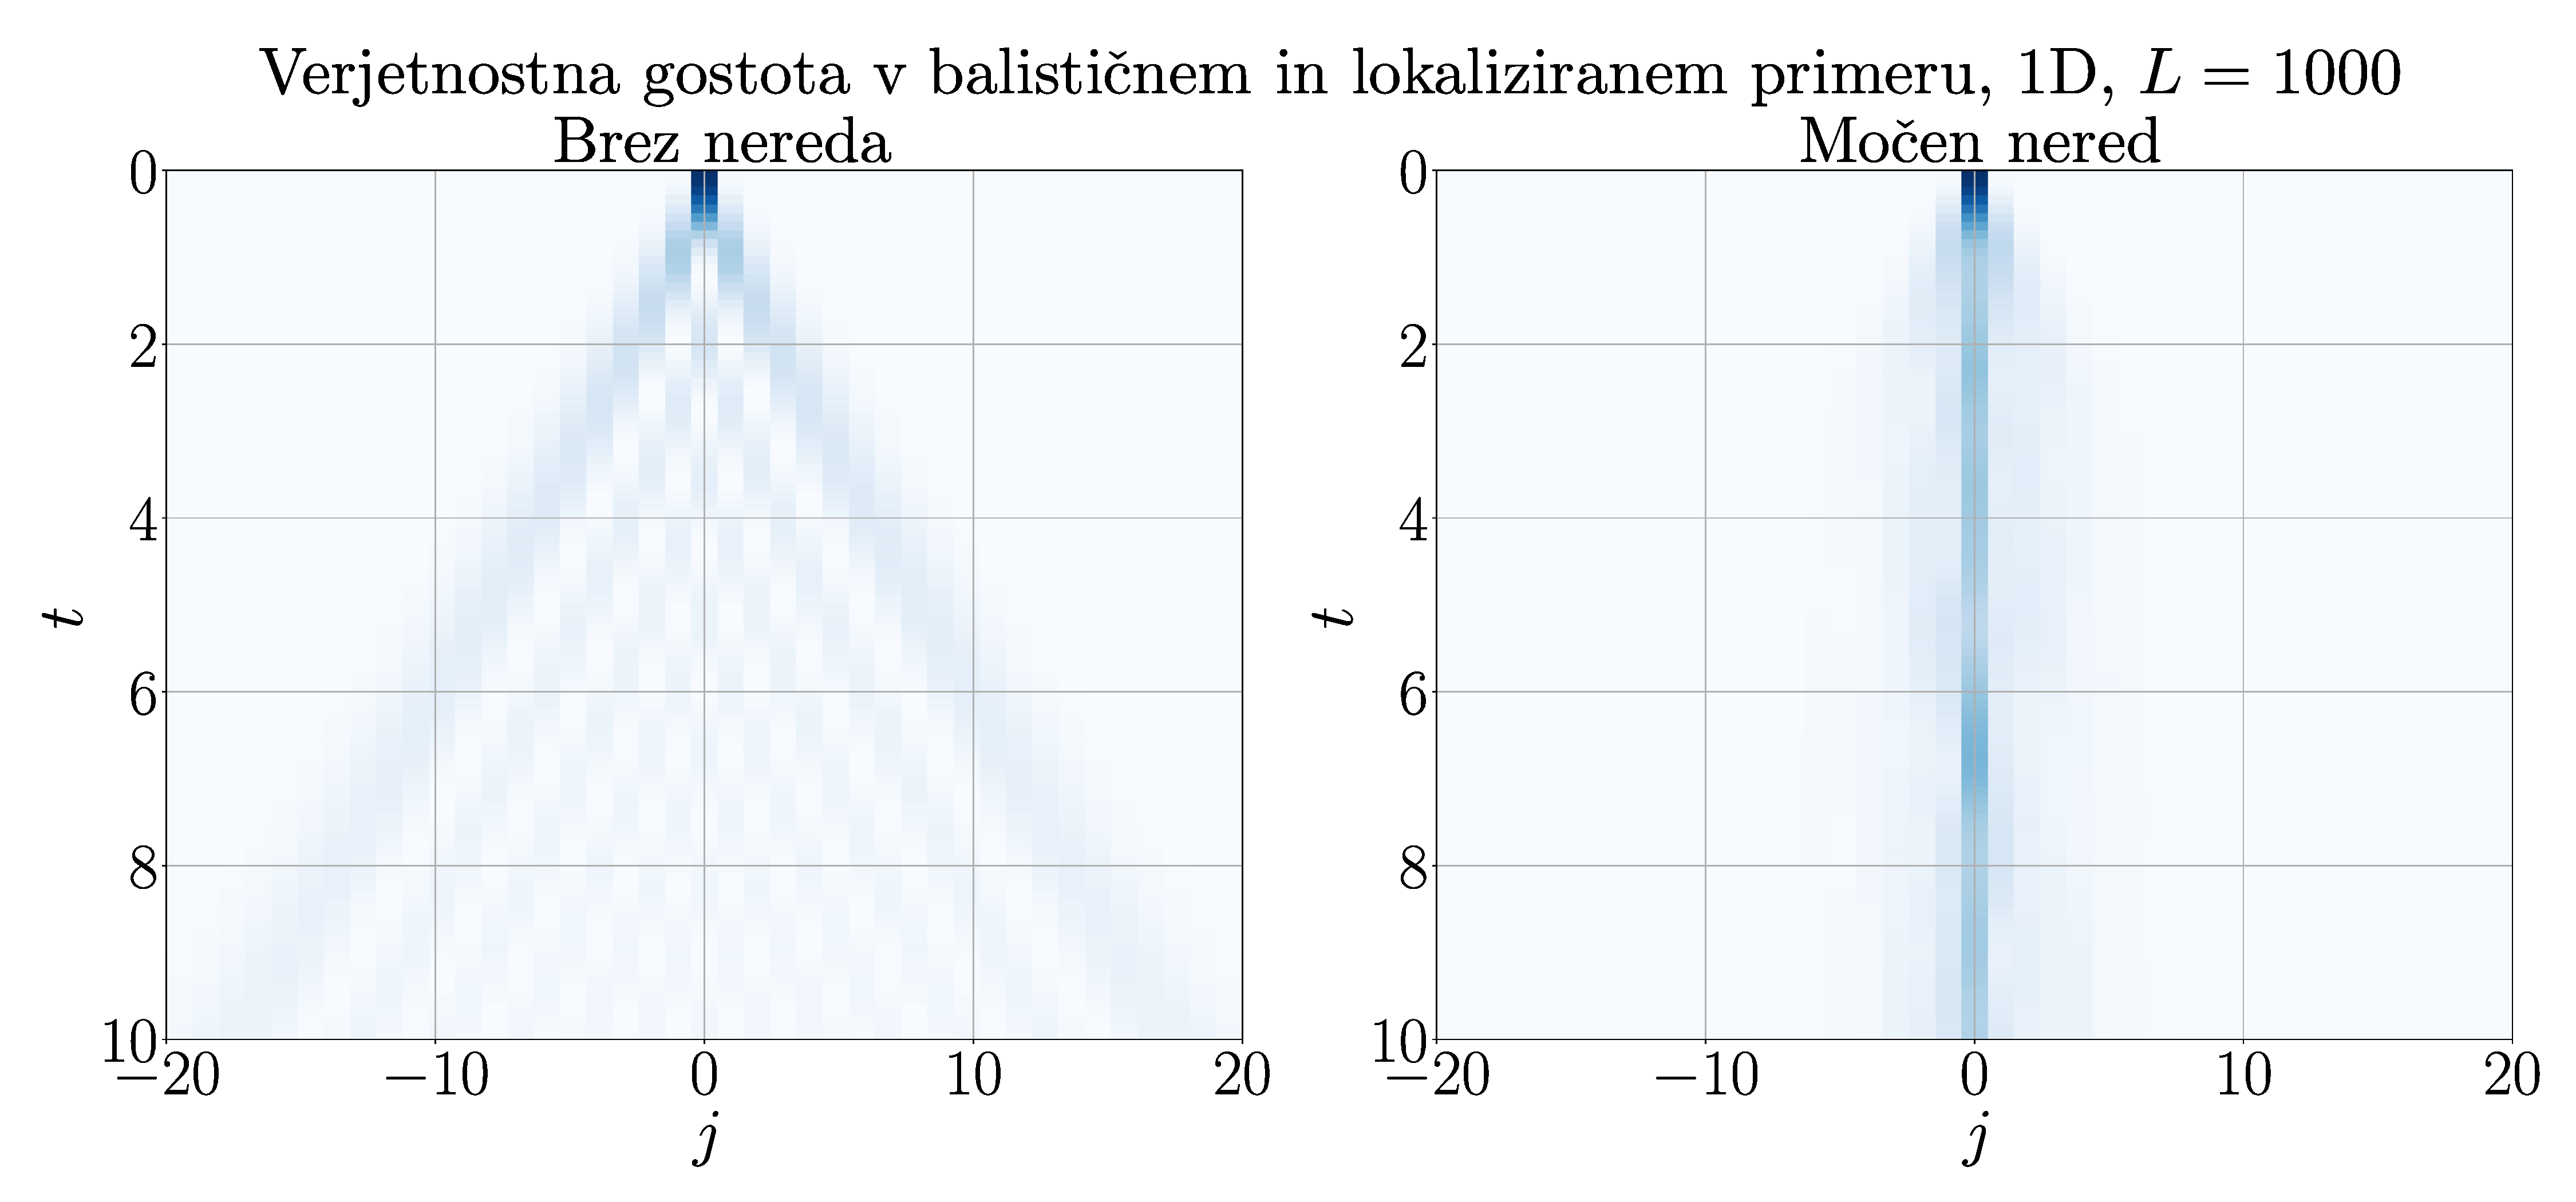
\includegraphics[width=0.8\textwidth]{1D_Anderson_localization_Seminar_scaling_analysis_D1_shape_1000_light_cone_double_presentation.pdf}}
\end{figure} 
\subsection{Lokalizacija v sistemih z meddelčnimi interakcijami}
Do sedaj smo se ukvarjali z lokalizacijo v sistemih neinteragirajočih delcev. Pri opisu dejanskih sistemov predstavlja predpostavka odsotnosti meddelčnih interakcij glavno pomanjkljivost modelov enodelčne lokalizacije. V praksi so namreč interakcije vselej prisotne, njihov vpliv pa vse od Andersonovega prelomnega članka ostaja eno pomembnejših odprtih vprašanj področja. Polno lokaliziran Andersonov izolator brez roba mobilnosti namreč pri nobeni temperaturi ne omogoča transporta energije ali naboja in tako zaradi ničelne prevodnosti vselej preprečuje termalizacijo. Da bi v interagirajočih sistemih lahko z gotovostjo potrdili oziroma ovrgli odsotnost termalizacije in nastop večdelčne lokalizacije, moramo v dosedanjo obravnavo neinteragirajočih sistemov neizogibno vključiti meddelčne interakcije in preučiti njihov vpliv. Zavoljo pregleda nad raziskovalno dejavnostjo in za lažjo umestitev v časovni okvir je na tem mestu navedenih nekaj zgodovinsko pomembnejših del s področja, v katerih je bil obravnavan preplet interakcij in nereda. Pri tem sledimo Ref.~\cite{abanin2018ergodicity}.\\\\
Leta 1980 sta Fleishman in Anderson~\cite{fleishman1980interactions} podala kvalitativne argumente v prid nastopu lokalizacije ob prisotnosti šibkih interakcij kratkega dosega. Uporaba teorije renormalizacijske grupe je omogočila posplošitev koncepta Andersonovega izolatorja in posledično opis osnovnih stanj neurejenih sistemov z interakcijami. V ta okvir spada delo Finkelsteina~\cite{finkelshtein1983influence}, ki je leta 1983 pri nadgraditvi skalirne teorije lokalizacije upošteval preplet vpliva meddelčnih interakcij in nereda. Mnogo kasneje so se pojavile utemeljitve obstoja lokalizirane faze ob prisotnosti interakcij pri \emph{končnih} temperaturah. Med prvimi so na to možnost leta 1997 pokazali Altshuler in sodelavci~\cite{altshuler1997quasiparticle} na primeru ničdimenzionalne kvantne pike. Obstoj lokalizacije v višjedimenzionalnih sistemih z lokalnimi interakcijami so leta 2006 utemeljili Basko, Aleiner in Altshuler~\cite{basko2006metal}, in sicer za nizke temperature oziroma nizke energijske gostote. V Ref.~\cite{basko2006metal} uporabljeni modelski sistem je namreč idealen izolator z ničelno prevodnostjo pri nizkih energijskih gostotah, medtem ko postanejo večdelčna lastna stanja pri visokih energijskih gostotah delokalizirana. To označuje fazni prehod med izolatorsko in prevodno fazo, ki nastopi pri končni temperaturi, oziroma točneje, pri končni energijski gostoti nad osnovnim stanjem, poimenovani \emph{večdelčni rob mobilnosti}. Fazni prehod v večdelčno lokalizirano stanje je kvalitativno drugačen od konvencionalnih končnotemperaturnih prehodov med kovino in izolatorjem v Mottovih in pasovnih izolatorjih. V slednjih je namreč specifična prevodnost pri končni temperaturi končna, vendar eksponentno majhna, medtem ko je v nizkotemperaturnem režimu večdelčno lokalizirane faze \emph{identično} enaka nič~\cite{basko2006problem}. Obstoj večdelčno lokalizirane faze tudi pri neskončni temperaturi v neurejenem interagirajočem sistemu na diskretni mreži sta leta 2007 utemeljila Oganesyan in Huse~\cite{PhysRevB.75.155111}, in sicer na podlagi numerične analize enodimenzionalnega modela s fermioni brez spinskih prostostnih stopenj. Z uporabo polne diagonalizacije modelskih hamiltonk in študijo spektralnih statistik sta prišla do rezultatov, ki napovedujejo obstoj večdelčno lokalizirane faze v neurejenih modelih na diskretnih mrežah tudi ob neskončnih temperaturah oziroma pri energijskih gostotah visoko nad osnovnim stanjem. Napoved velja za sisteme s končnodimenzionalnimi lokalnimi Hilbertovimi prostori, torej sisteme s končnim številom stanj na mesto. 
Članek je navdahnil številne kasnejše numerične raziskave MBL pojavov, po njem pa se pri analizi spektralnih statistik v magistrski nalogi obravnavanih modelov zgledujemo tudi mi.
\\\\ 
Čeprav koncepti v podpoglavju~\ref{anderson} obravnavane Andersonove lokalizacije služijo kot izhodišče za obravnavo fenomenov večdelčne lokalizacije, se problema bistveno razlikujeta. Interakcije v interagirajočih večdelčnih sistemih sklapljajo različna mnogodelčna stanja. V kolikor v sistemu obstajajo delokalizirana stanja, lahko interakcije denimo omogočijo prehod iz lokaliziranega osnovnega stanja v vzbujeno delokalizirano večdelčno stanja in povzročijo fazni prehod med izolativnim in prevodnim obnašanjem. Pri presoji obstoja večdelčno lokalizirane faze moramo tako preučiti naravo vseh mnogodelčnih lastnih stanj sistema in ugotoviti, ali so lokalizirana ali ne. Ker preučujemo stanja s končnimi energijskimi gostotami nad energijo osnovnega stanja, nas zanimajo končne temperature. Na drugi strani nas zaradi odsotnosti meddelčnih interakcij pri Andersonovem izolatorju v resnici zanimata le osnovno stanje in končno število vzbuditev nad njim. V termodinamski limiti neskončnega sistema je energijska gostota vzbuditev enaka nič, kar ustreza ničelni temperaturi. 
\\\\
V nadaljevanju razložimo osnovne koncepte fizike zaprtih kvantnih sistemov. Ker je poglavitna lastnost MBL sistemov odsotnost termalizacije, je zatem podrobneje predstavljen mehanizem termalizacije v kvantnih sistemih skupaj s \emph{hipotezo termalizacije lastnih stanj} (ang. \emph{eigenstate thermalization hypothesis}, v nadaljevanju ETH). Nazadnje so navedene najpomembnejše značilnosti MBL sistemov. 
\subsubsection{Fizika zaprtih kvantnih sistemov}
Pojav MBL se tipično preučuje v zaprtih kvantnih sistemih, kjer zaprtost pomeni odsotnost sklopitve z okolico oziroma zunanjim rezervoarjem. V tem podpoglavju navedemo osnovne koncepte, ki določajo obnašanje tovrstnih sistemov. V razpravi imamo vselej v mislih časovno neodvisne hamiltonke z interakcijami kratkega dosega. 
% \paragraph{Unitaren časovni razvoj kvantnih sistemov}
Ker se pri obravnavi ne omejujemo izključno na čista stanja, opisuje poljubno stanje zaprtega kvantnega sistema gostotna matrika, $\hat{\rho}(t)=\ket{\psi(t)}\bra{\psi(t)}$. V Schrödingerjevi sliki, kjer je časovni razvoj poljubnega začetnega stanja določen z delovanjem unitarnega časovnega propagatorja, 
\begin{equation}\label{eq:cas_razvoj}
\ket{\psi(t)}=\mathrm{e}^{-\iu \hat{H} t}\ket{\psi(0)},
\end{equation}
 je časovni razvoj gostotne matrike določen z zvezami 	
\begin{equation}
\hat{\rho}(t)=\mathrm{e}^{\iu \hat{H} t}\hat{\rho}(0)\ \mathrm{e}^{-\iu \hat{H} t}, \hspace{5mm} \iu\hbar\frac{\dd \hat{\rho}}{\dd t}=\left[\hat{H}, \hat{\rho}\right]; \hspace{5mm} \Tr{\hat{\rho}}=1.
\end{equation}
Vsi drugi kvantnomehanski operatorji $\hat{O}$ so časovno neodvisni, pričakovana vrednost poljubnemu operatorju $\hat{O}$ pripadajoče opazljivke $O$ pa se ob času $t$ zapiše kot 
\begin{equation}
\langle \hat{O}\rangle_t = \Tr\left(\hat{O}\hat{\rho}(t)\right).
\end{equation}
V klasični statistični mehaniki temelji koncept termalizacije na predpostavki \emph{ergodičnosti}, v skladu s katero so na dolgem časovnem intervalu vsa mikrostanja sistema obiskana z enako verjetnostjo. Zaradi linearnosti kvantne mehanike moramo v kvantnih sistemih pojem ergodičnosti nekoliko prilagoditi. Vzemimo namreč poljubno začetno neravnovesno stanje večdelčnega sistema $\ket{\psi(0)}$ in ga razvijmo po bazi večdelčnih lastnih stanj $\ket{\alpha}$ kot $\ket{\psi(0)}=\sum\limits_\alpha A_\alpha \ket{\alpha}$. Pri časovnem razvoju v skladu z En.~\ref{eq:cas_razvoj} pridobi vsak izmed koeficientov razvoja $A_\alpha$ multiplikativni fazni faktor, ki ustreza dani večdelčni lastni energiji $E_\alpha$, 
$$
\ket{\psi(t)}=\mathrm{e}^{-\iu \hat{H} t}\ket{\psi(0)}=\sum\limits_\alpha A_\alpha \mathrm{e}^{-\iu E_\alpha t}\ket{\alpha}.
$$
Verjetnost $p_\alpha$, da se sistem nahaja v enem izmed lastnih stanj $\ket{\alpha}$, se s časom seveda ne spreminja in je določena z začetno izbiro stanja, saj velja $p_\alpha=\abs{A_\alpha}^2$. To je popolnoma drugače kot v klasičnih sistemih, ki med časovnim razvojem obiščejo različne dele faznega prostora. V kvantnih sistemih se pojem termalizacije namesto na same valovne funkcije	ali gostotne matrike nanaša na pričakovane vrednosti \emph{lokalnih} opazljivk po dolgem času, ki jih podaja izraz~\cite{deutsch1991quantum}~\cite{abanin2018ergodicity}
\begin{equation}\label{eq:ergodicnost_kvantno}
\langle \hat{O}\rangle_\infty=\lim_{t'\to\infty}\frac{1}{t'}\int\limits_0^{t'} \bra{\psi(t)}\hat{O}\ket{\psi(t)}\dd t = \sum\limits_\alpha p_\alpha\bra{\alpha}\hat{O}\ket{\alpha}.
\end{equation}
Iz En.~\eqref{eq:ergodicnost_kvantno} vidimo, da vrednost $\langle \hat{O}\rangle_\infty$ določajo verjetnosti $p_\alpha$ skupaj s pričakovanimi vrednostmi opazljivke $\bra{\alpha}\hat{O}\ket{\alpha}$. Izvendiagonalni matrični elementi v zgornji enačbi oscilirajo pri različnih frekvencah in se pri časovni integraciji v procesu \emph{dekoherence} izpovprečijo, hkrati pa smo na zadnjem koraku privzeli, da lastna stanja sistema niso degenerirana.	
Pri tem moramo dodati, da zaradi posledic efektov končnih velikosti sistemov $\langle\hat{O}\rangle_\infty$ doseže ravnovesno vrednost samo v termodinamski limiti neskončnega sistema, kjer moramo v En.~\eqref{eq:ergodicnost_kvantno} limito neskončnega sistema izvesti hkrati z limito $t\to\infty.$  Za končne sisteme je časovna dinamika namreč kvaziperiodična in tako dolgočasovna limita ni dobro definirana, medtem ko po končnem času difuzivna propagacija v termalizirajočem sistemu doseže le končen delež neskončnega sistema~\cite{PhysRevB.75.155111}. 
% \subsubsection{Termalizacija v zaprtih kvantnih sistemih}
% Intuitivno si lahko mislimo, da zaprt kvantni sistem termalizira, če se za fizikalno začetno stanje po dovolj dolgem času pričakovane vrednosti opazljivk, dane z En.~\eqref{eq:ergodicnost_kvantno}, ujemajo z ustreznimi ansambelskimi povprečji - v limiti neskončnega sistema dobimo v mikrokanoničnem, kanoničnem in velekanoničnem ansamblu enake rezultate. S fizikalnimi stanji mislimo na eksperimentalno dosegljiva stanja, kot so denimo produktna stanja ali superpozicije ekstenzivno mnogo lastnih funkcij, medtem ko posamezne lastne funkcije ne predstavljajo fizikalnih stanj. Čas, potreben za njihovo pripravo namreč skalira eksponentno z velikostjo sistema~\cite{abanin2018ergodicity}.\\\\
% Ravnovesno stanje kvantnega sistema popolnoma določa nekaj makroskopskih parametrov, kot sta denimo temperatura in kemijski potencial - v splošnem se število parametrov ujema s številom ekstenzivnih ohranjenih količin sistema. V nadaljevanju podpoglavja bomo brez škode za splošnost privzeli obravnavo sistema, v katerem je ekstenzivna ohranjena količina zgolj energija, tako da v primeru termalizacije celoten sistem opiše le en parameter, in sicer temperatura. Pri iskanju odgovora na vprašanje, kaj v odsotnosti sklopitve z rezervoarjem termalizacijo sploh omogoča, je sistem ugodno razdeliti na dva podsistema. V manjšem podsistemu A naj bo makroskopsko zanemarljiv delež prostostnih stopenj celotnega sistema, preostanek sistema pa predstavlja podsistem B. Hamiltonka mora pri tem prostostne stopnje celotnega sistema sklapljati tako, da ne obstajajo podsistemi, ko se sami ne sklapljajo s preostankom sistema in so od njega izolirani. V primeru termalizacije je po dolgem času podsistem A v ravnovesnem stanju, kot bi bil sklopljen z rezervoarjem pri temperaturi $T$. Naš namišljeni rezervoar je v resnici kar preostanek sistema - termalizacija in relaksacija začetnih stanj proti ravnovesnim stanjem sta v zaprtih kvantnih sistemih namreč možni, če lahko sistemi svojim podsistemom služijo kot rezervoarji. Nekoliko formalneje zgoraj povedano zapišemo z uporabo gostotne matrike $\hat{\rho}_\mathrm{A}$ za podsistem A, ki jo ob času $t$ iz gostotne matrike celotnega sistema dobimo z delno sledjo po prostostnih stopnjah podsistema B:
% \begin{equation}
% \hat{\rho}_\mathrm{A}(t)= \mathrm{Tr}_\mathrm{B}\left\{\hat{\rho}(t)\right\}.
% \end{equation}
% Ravnovesna gostotna matrika celotnega sistema je pri temperaturi $T$ podana z Boltzmannovim operatorjem, medtem ko ravnovesno gostotno matriko podsistema A ponovno dobimo z delno sledjo po podsistemu B, torej
%  \begin{equation}\hat{\rho}^\mathrm{(eq)}(T)=Z^{-1}(T)\exp\left(-\hat{H}/k_\mathrm{B}T\right),\hspace{5mm} \hat{\rho}_\mathrm{A}^\mathrm{(eq)}(T)=\mathrm{Tr}_\mathrm{B}\left\{\hat{\rho}^{(\mathrm{eq})}(T)\right\}.
%  \end{equation}
% Termalizacija pri temperaturi $T$ nastopi, če v hkrati vzetih limitah neskončnega sistema in neskončnega časa za vse možne 	izbire podsistemov A velja 
% \begin{equation}
% \hat{\rho}_\mathrm{A}(t)=\hat{\rho}_\mathrm{A}^{(\mathrm{eq})}(T).
% \end{equation}

\subsubsection{Termalizacija in hipoteza termalizacije lastnih stanj}
Termalizacija v jeziku konvencionalne statistične fizike pomeni relaksacijo vseh, še tako neravnovesnih, stanj proti ravnovesju, v katerem pričakovane vrednosti opazljivk določajo ustrezna ansambelska povprečja. Poljubna začetna stanja z izbrano energijo v termalizirajočem sistemu vsa termalizirajo pri temperaturi $T$, ustrezajoči pričakovani vrednosti energije sistema po dolgem času $\langle\hat{H}\rangle_T$, kjer smo seveda privzeli ohranitev celotne energije sistema. Pri posplošitvi obravnave na zaprte kvantne sisteme predpostavimo da tudi v teh, v kolikor pride do termalizacije, vsa začetna stanja z dano energijo termalizirajo pri isti temperaturi. Izjava je splošna in do zdaj rigorozen dokaz trditve za splošne generične sisteme še ne obstaja, vendar se zdi v skladu s tem, kar vemo o naravi termalizirajočih sistemov~\cite{nandkishore2015many}.\\\\
Če sistem za vsako začetno stanje $\hat{\rho}(0)$ z dano energijo resnično termalizira pri ustrezni temperaturi, potem je zaradi enostavne časovne dinamike  ugodno obravnavati  mnogodelčna lastna stanja hamiltonke sistema, $\hat{H}\ket{\alpha}=E_\alpha\ket{\alpha}$. Časovni razvoj začetne gostotne matrike sistema $\hat{\rho}(0)=\ket{\alpha}\bra{\alpha}$, je v tem primeru trivialen, namreč $\hat{\rho}(t)=\hat{\rho}(0)$. V kolikor je zgoraj omenjena predpostavka termalizacije vseh začetnih stanj upravičena, potem so lastna stanja hamiltonke že sama po sebi termalna. Domnevo imenujemo \emph{hipoteza termalizacije lastnih stanj}~\cite{deutsch1991quantum}~\cite{srednicki1999approach} (ang. \emph{eigenstate thermalization hypothesis}, v nadaljevanju ETH).
Imejmo začetno čisto stanje $\ket{\psi(0)}$ z dobro definirano povprečno energijo $\bar{E}$ in majhnimi fluktuacijami $\Delta$, $\Delta\ll\bar{E}$. To pomeni, da je $\ket{\psi}$ superpozicija lastnih stanj znotraj energijskega okna $\Delta$. Velja~\cite{srednicki1999approach}
\begin{equation}
\begin{split}
\ket{\psi}&=\sum\limits_\alpha A_\alpha\ket{\alpha}, \\
\bar{E}&=\sum\limits_\alpha \abs{A_\alpha}^2E_\alpha, \\
\Delta^2&=\sum\limits_\alpha \abs{A_\alpha}^2\left(E_\alpha - \bar{E}\right).
\end{split}
\end{equation}
ETH napove, da za izbrano začetno stanje $\ket{\psi(0)}$ po dolgem času pričakovane vrednosti lokalnih operatorjev $\hat{O}$ relaksirajo proti ravnovesnim vrednostim mikrokanoničnega ansambla pri energiji $\bar{E}.$ Ob veljavnosti ETH se slednje ujemajo s pričakovanimi vrednostmi $\hat{O}$ v tipičnih lastnih stanjih $\ket{\alpha}_\mathrm{Typ}$ znotraj energijskega okna $\Delta$ okrog $\bar{E}$. En.~\eqref{eq:ergodicnost_kvantno} tako prepišemo kot
\begin{equation}
\langle \hat{O}\rangle_\infty=\lim_{t\to\infty}\bra{\psi(t)}\hat{O}\ket{\psi(t)}=\frac{\sum_{\abs{E_\alpha - \bar{E}}\leq \Delta}\bra{\alpha}\hat{O}\ket{\alpha}}{N_\Delta}=_\mathrm{Typ}\bra{\alpha}\hat{O}\ket{\alpha}_\mathrm{Typ}.
\end{equation}
S tipičnim stanjem imamo v resnici v mislih katerokoli lastno stanje znotraj energijskega okna, pri čemer je $N_\Delta$ število lastnih stanj na danem enerijskem intervalu. Bistvo zgornje enačbe in ETH nasploh je, da v termalizirajočem sistemu ravnovesne vrednosti opazljivk podajo kar pričakovane vrednosti v posameznih lastnih stanjih, katerih energija ustreza energiji sistema. \\\\
Veljavnost ETH v sistemu pomeni njegovo termalizacijo in tako implicira ergodičnost v kvantnem primeru. Podrobnim numeričnim študijam ETH navkljub~\cite{d2016quantum} trenutno še ni povsem jasno, ali je veljavnost hipoteze potreben pogoj za termalizacijo - za zdaj vemo zgolj, da ETH velja v vseh termalizirajočih sistemih. Hipoteza ni veljavna v dveh pomembnih razredih netermalizirajočih sistemov. V integrabilnih sistemih relaksacijo proti termalnim vrednostim preprečuje nabor konstant  gibanja. Kljub temu lahko v integrabilnih sistemih pričakujemo relaksacijo proti stanjem z maksimalno entropijo in posplošeno verzijo termalizacije proti t.i. generaliziranemu Gibbsovemu ansamblu. Drugi tip sistemov so za nas zanimivejši MBL sistemi, ki jih zaznamuje odsotnost termalizacije v kakršnemkoli smislu. 
\subsubsection{Značilnosti MBL sistemov } 
MBL sistemi se v več pogledih ločijo od termalizirajočih oziroma ergodičnih sistemov. V tem poglavju na kratko predstavimo nekaj njihovih poglavitnih lastnosti, in sicer neergodičnost v času, značilno spektralno statistiko, ničelni transport ter skaliranje prepletenostne entropije. \\\\	
Kot smo opisali v predhodnem poglavju, so v ergodičnih sistemih večdelčna lastna stanja termalna, kar v izoliranem sistemu dovoljuje relaksacijo poljubnega začetnega stanja proti ravnovesni vrednosti - sistem lahko \emph{sam sebi služi kot toplotna kopel}. V MBL sistemih je drugače, saj zanje ETH ne velja in lastna stanja niso termalna. Tudi po dolgem času so pričakovane vrednosti lokalnih opazljivk namesto s termalnimi vrednostmi določene s podrobnostmi lokalnih konfiguracij začetnih stanj. Začetna stanja se z gostotno matriko v bazi lastnih stanj zapišejo kot $\hat{\rho}=\sum\limits_{\alpha,\beta}\rho_{\alpha\beta}\ket{\alpha}\bra{\beta}.$ V ergodičnem primeru se vsa informacija o prekrivanju začetnega stanja z lastnimi funkcijami sistema po dolgočasovnem razvoju porazgubi, oziroma točneje rečeno, preplete s preostalimi lokalnimi prostostnimi stopnjami. Izvendiagonalni matrični elementi se zaradi dekoherence namreč kot v En.~\eqref{eq:ergodicnost_kvantno} po dolgem času izpovprečijo, diagonalni elementi pa ostanejo nespremenjeni. Ker so lastna stanja v ergodičnem primeru termalna, vodi unitarna hamiltonska dinamika do termalnega ravnovesja. V MBL primeru dekoherenca izvendiagonalnih matričnih elementov sicer tudi zabriše informacijo o naravi začetnega stanja, 
vendar se slednja ohrani v diagonalnih elementih gostotne matrike. Ker v MBL primeru lastna stanja niso termalna, so diagonalni matrični elementi namreč določeni z lokalnimi značilnostmi lastnih stanj.\\\\
Neergodičnost MBL sistemov se odraža tudi v lastnostih energijskih spektrov njihovih hamiltonk, 
%TO DO: 
%KAJ NAJ BO V UVODU: -> GIBALNE ENAČBE ZA VEČDELČNE SISTEME (VON NEUMANN) CHECK
%RAZLAGA IZOLACIJE IN KAJ JE SPLOH ERGODIČNOST V KVANTNEM SISTEMU (GLEJ D ALLESSIO) CHECK
%INTERAKCIJE -> POMEN: KONČNA GOSTOTA ENERGIJE, KAKO JE TO DRUGAČE OD ANDERSONA -> daj to najprej po uvodnem odstavku, VIRI: Basko, Oganesyan, Huse, CHECK

%NAJPREJ ZA UVOD: ETH, INTEGRABILNI, MBL -> 4 lastnosti: STATISTIKA, NEERGODIČNOST V ČASU , TRANSPORT 0, ENTENGLEMENT ŠE TREBA
%ENAČBE ZA ZAPRTE KVANTNE SISTEME -> ČASOVNI RAZVOJ:  CHECK
%Nandkishore, Huse: kje se to lahko študira: sistemi z mobilnimi delci, glej poglavje 4.2
\newpage
\section{Modeli}
V poglavju predstavimo modele, v katerih 
\subsection{Heisenbergova veriga}
\subsection{Hubbardov model}
\subsection{Model t-J}
\subsection{Točna diagonalizacija}
\section{Statistične lastnosti hamiltonskih spektrov}
\subsection{Statistika sosednjih energijskih nivojev}
\subsection{Spektralni oblikovni faktor}	
\section{Prepletenostna entropija}



\newpage
\bibliographystyle{fmf-sl}
\bibliography{literatura}




\end{document}


